% ============================================================================
% Report 2 of 2: results of the filmed tests.
%
% Data sections are generated from the CSVs exported by VidFetch (see informe_aplicacion.tex,
% section "Procedimiento"), from the repository root:
%   python software/vidfetch/tools/reexportar.py datos/video/sesiones/VA_<código>_analisis.npz ...   (optional)
%   python software/analisis_video/generar_informe.py datos/video/trayectorias/VP_<código>_robots.csv \
%          --video datos/video/recortados/VC_<código>.MP4 --nombre <código>
%   python software/analisis_video/comparar_ensayos.py "datos/video/trayectorias/VP_*_robots.csv"
% Then compile this file twice. Hand-written text: secciones/*.tex.
% ============================================================================
\documentclass[11pt, a4paper]{article}
% ----------------------------------------------------------------------------
% Preamble: packages, language, units, colours and PGFPlots styles.
% ----------------------------------------------------------------------------
\usepackage[T1]{fontenc}
\usepackage[utf8]{inputenc}
\IfFileExists{lmodern.sty}{\usepackage{lmodern}}{}
\usepackage[a4paper, margin=2.3cm]{geometry}

% Spanish when available (TeX Live full / MiKTeX); otherwise English babel + Spanish names.
\IfFileExists{spanish.ldf}{%
  \usepackage[spanish, es-noshorthands, es-tabla]{babel}%
}{%
  \usepackage[english]{babel}%
  \addto\captionsenglish{%
    \renewcommand{\figurename}{Figura}\renewcommand{\tablename}{Tabla}%
    \renewcommand{\contentsname}{Índice}\renewcommand{\refname}{Referencias}%
  }%
}

\emergencystretch=2em   % avoid overfull lines with long \texttt file names
\usepackage{amsmath, amssymb}
\usepackage{graphicx}
\usepackage{float}
\usepackage{booktabs}
\usepackage{caption}
\captionsetup{font=small, labelfont=bf}
\usepackage{xcolor}

\usepackage{siunitx}
% Numbers arrive already rounded by generar_informe.py: no re-rounding (integers stay integers).
\sisetup{output-decimal-marker = {,}, group-separator = {\,}, group-minimum-digits = 5,
         round-mode = none, per-mode = symbol}
\DeclareSIUnit{\px}{px}

\usepackage{tikz}
\usetikzlibrary{positioning, fit, backgrounds, calc}
\usepackage{pgfplots}
\usepackage{pgfplotstable}
\pgfplotsset{compat=1.17}
\usepgfplotslibrary{fillbetween}
\pgfkeys{/pgf/number format/.cd, use comma, 1000 sep={\,}}

% Time-scale helpers: every frame <-> real-time equivalence in the text is computed from
% \CuadrosPorSegundo (config.tex), so changing that single value updates the whole report.
\newcommand{\FileFps}{29.97}   % playback rate of the DJI files [frames/s]
\newcommand{\CalcNum}[2][3]{\pgfmathsetmacro\calcres{#2}\num[round-mode=figures, round-precision=#1]{\calcres}}
\newcommand{\CalcQty}[3][2]{\pgfmathsetmacro\calcres{#2}\SI[round-mode=figures, round-precision=#1]{\calcres}{#3}}
\newcommand{\EnSeg}[1]{\CalcQty{#1/\CuadrosPorSegundo}{\second}}          % n frames -> real seconds
\newcommand{\Cuadros}[1]{\num{#1}~cuadros (\EnSeg{#1})}                    % "n cuadros (x s)"
\newcommand{\fr}{f_{\mathrm{r}}}
\newcommand{\fa}{f_{\mathrm{a}}}

\definecolor{azul}{RGB}{42,111,219}
\definecolor{rojo}{RGB}{211,51,51}
\definecolor{verde}{RGB}{34,160,60}
\definecolor{naranja}{RGB}{240,140,0}

% Cycle of 12 distinguishable colours for per-robot curves (repeats beyond 12 robots).
\pgfplotscreateplotcyclelist{robots}{
  {color=azul}, {color=rojo}, {color=verde}, {color=naranja}, {color=violet}, {color=teal},
  {color=brown}, {color=magenta}, {color=olive}, {color=cyan!70!black}, {color=gray}, {color=black}}

% Code listings (application report). Comments in the code are in English.
\usepackage{listings}
\definecolor{codefondo}{RGB}{246,247,249}
\definecolor{codecom}{RGB}{110,120,130}
\definecolor{codekw}{RGB}{42,111,219}
\definecolor{codestr}{RGB}{170,80,20}
\lstdefinestyle{py}{language=Python, basicstyle=\ttfamily\footnotesize, keywordstyle=\color{codekw}\bfseries,
  commentstyle=\color{codecom}\itshape, stringstyle=\color{codestr}, backgroundcolor=\color{codefondo},
  frame=single, rulecolor=\color{gray!40}, framesep=4pt, xleftmargin=6pt, xrightmargin=6pt,
  numbers=left, numberstyle=\tiny\color{gray}, numbersep=6pt, breaklines=true, showstringspaces=false,
  columns=fullflexible, keepspaces=true, upquote=true, tabsize=4, captionpos=b,
  literate={á}{{\'a}}1 {é}{{\'e}}1 {í}{{\'i}}1 {ó}{{\'o}}1 {ú}{{\'u}}1 {ñ}{{\~n}}1 {θ}{{$\theta$}}1 {ω}{{$\omega$}}1}
\lstset{style=py}
\renewcommand{\lstlistingname}{Código}
\renewcommand{\lstlistlistingname}{Índice de códigos}

\usepackage[hidelinks]{hyperref}
\usepackage{cleveref}
% Spanish reference names regardless of the babel language actually loaded.
\crefname{figure}{fig.}{figs.}\Crefname{figure}{Figura}{Figuras}
\crefname{table}{tabla}{tablas}\Crefname{table}{Tabla}{Tablas}
\crefname{section}{sección}{secciones}\Crefname{section}{Sección}{Secciones}
\crefname{subsection}{sección}{secciones}\Crefname{subsection}{Sección}{Secciones}
\crefname{lstlisting}{código}{códigos}\Crefname{lstlisting}{Código}{Códigos}\crefname{listing}{código}{códigos}\Crefname{listing}{Código}{Códigos}
\crefname{equation}{ec.}{ecs.}\Crefname{equation}{Ecuación}{Ecuaciones}
\creflabelformat{equation}{(#2#1#3)}

% ----------------------------------------------------------------------------
% Experiment-wide settings. Edit here; every section reads these macros.
% ----------------------------------------------------------------------------
% Titles of the two reports (informe_aplicacion.tex and informe_ensayos.tex).
\newcommand{\TituloAplicacion}{VidFetch: seguimiento de robots en video}
\newcommand{\SubtituloAplicacion}{Uso, funcionamiento y código de la aplicación}
\newcommand{\TituloEnsayos}{Robots autopropulsados confinados: resultados de los ensayos filmados}
\newcommand{\SubtituloEnsayos}{Posición, velocidad, rotación y atascos en tres ensayos con 22 robots}
\newcommand{\Autores}{Dylan Frigerio}
\newcommand{\Institucion}{ITBA}
\newcommand{\FechaInforme}{\today}

% Real robot diameter (same value as "Diámetro real" in the app; 33 mm, consistent with the image
% measured with the enclosure scale). It sets the wall-contact radius and the area fraction, not the scale.
\newcommand{\DiametroRobotCM}{3.3}

% Enclosure (recinto): inner and outer diameter of the wall ring. The px -> mm scale of every frame
% comes from the inner diameter (same values as "Diámetro interior/exterior" in the app).
\newcommand{\DiametroIntRecintoCM}{18.5}
\newcommand{\DiametroExtRecintoCM}{19.5}

% Time scale of the time-lapse videos: frames that correspond to 1 s of real time
% (same value as "Escala de tiempo" in the app; 3 by default).
\newcommand{\CuadrosPorSegundo}{3}


\title{\TituloEnsayos\\[2pt]\large \SubtituloEnsayos}
\author{\Autores \\ \small \Institucion}
\date{\FechaInforme}

\IfFileExists{generado/comparacion/datos.tex}{% Generated by comparar_ensayos.py -- do not edit; re-run the script instead.
\expandafter\def\csname CmpCodA\endcsname{20262409\_1600\_22QR\_60}
\expandafter\def\csname CmpLabA\endcsname{24/09 16:00}
\expandafter\def\csname CmpNA\endcsname{22}
\expandafter\def\csname CmpFA\endcsname{12069}
\expandafter\def\csname CmpFpsA\endcsname{3}
\expandafter\def\csname CmpDurA\endcsname{67}
\expandafter\def\csname CmpEscA\endcsname{0.323}
\expandafter\def\csname CmpRarA\endcsname{9.25}
\expandafter\def\csname CmpPhiA\endcsname{0.7}
\expandafter\def\csname CmpRcA\endcsname{77.8}
\expandafter\def\csname CmpRcRelA\endcsname{0.841}
\expandafter\def\csname CmpKapA\endcsname{0.977}
\expandafter\def\csname CmpDmmA\endcsname{33}
\expandafter\def\csname CmpMovXA\endcsname{1.58}
\expandafter\def\csname CmpMovYA\endcsname{4.1}
\expandafter\def\csname CmpZoomA\endcsname{0.938}
\expandafter\def\csname CmpRatioRA\endcsname{1.05}
\expandafter\def\csname CmpResRA\endcsname{0.984}
\expandafter\def\csname CmpPwallA\endcsname{56}
\expandafter\def\csname CmpPwallCcwA\endcsname{64.9}
\expandafter\def\csname CmpPwallCwA\endcsname{51.7}
\expandafter\def\csname CmpPcwCcwA\endcsname{49.1}
\expandafter\def\csname CmpWabsCcwA\endcsname{0.647}
\expandafter\def\csname CmpWabsCwA\endcsname{3.46}
\expandafter\def\csname CmpVtanA\endcsname{-1.04}
\expandafter\def\csname CmpObsA\endcsname{100}
\expandafter\def\csname CmpRelA\endcsname{216}
\expandafter\def\csname CmpIntA\endcsname{0}
\expandafter\def\csname CmpManA\endcsname{0}
\expandafter\def\csname CmpPreA\endcsname{0}
\expandafter\def\csname CmpVmedA\endcsname{0.502}
\expandafter\def\csname CmpVmeanA\endcsname{0.904}
\expandafter\def\csname CmpVp95A\endcsname{3.12}
\expandafter\def\csname CmpVmedActA\endcsname{0.643}
\expandafter\def\csname CmpWmedA\endcsname{3.06}
\expandafter\def\csname CmpWmeanA\endcsname{-2.81}
\expandafter\def\csname CmpWposA\endcsname{41.2}
\expandafter\def\csname CmpNccwA\endcsname{8}
\expandafter\def\csname CmpNcwA\endcsname{14}
\expandafter\def\csname CmpVmaxA\endcsname{163}
\expandafter\def\csname CmpVnetA\endcsname{-691}
\expandafter\def\csname CmpSpinA\endcsname{14.6}
\expandafter\def\csname CmpNAtA\endcsname{3}
\expandafter\def\csname CmpTAtA\endcsname{11.5}
\expandafter\def\csname CmpPAtA\endcsname{17.2}
\expandafter\def\csname CmpAtMaxA\endcsname{381}
\expandafter\def\csname CmpProtA\endcsname{-0.212}
\expandafter\def\csname CmpOmA\endcsname{-0.206}
\expandafter\def\csname CmpAlfaA\endcsname{1.35}
\expandafter\def\csname CmpMsdA\endcsname{8.94e+03}
\expandafter\def\csname CmpTauMaxA\endcsname{16.8}
\expandafter\def\csname CmpLagA\endcsname{20.7}
\expandafter\def\csname CmpRxcA\endcsname{0.549}
\expandafter\def\csname CmpLedA\endcsname{15.7}
\expandafter\def\csname CmpLedFinA\endcsname{20.7}
\expandafter\def\csname CmpLagLedA\endcsname{-0.0333}
\expandafter\def\csname CmpDesfA\endcsname{20.7}
\expandafter\def\csname CmpGinA\endcsname{876}
\expandafter\def\csname CmpGoutA\endcsname{0.0106}
\expandafter\def\csname CmpGratA\endcsname{82353}
\expandafter\def\csname CmpSatInA\endcsname{53.3}
\expandafter\def\csname CmpSatAllA\endcsname{9.15}
\expandafter\def\csname CmpHasSenA\endcsname{1}
\expandafter\def\csname CmpCodB\endcsname{20262509\_1230\_22QR\_60}
\expandafter\def\csname CmpLabB\endcsname{25/09 12:30}
\expandafter\def\csname CmpNB\endcsname{22}
\expandafter\def\csname CmpFB\endcsname{9881}
\expandafter\def\csname CmpFpsB\endcsname{3}
\expandafter\def\csname CmpDurB\endcsname{54.9}
\expandafter\def\csname CmpEscB\endcsname{0.324}
\expandafter\def\csname CmpRarB\endcsname{9.25}
\expandafter\def\csname CmpPhiB\endcsname{0.7}
\expandafter\def\csname CmpRcB\endcsname{78.2}
\expandafter\def\csname CmpRcRelB\endcsname{0.845}
\expandafter\def\csname CmpKapB\endcsname{0.972}
\expandafter\def\csname CmpDmmB\endcsname{33}
\expandafter\def\csname CmpMovXB\endcsname{1.48}
\expandafter\def\csname CmpMovYB\endcsname{3.28}
\expandafter\def\csname CmpZoomB\endcsname{0.36}
\expandafter\def\csname CmpRatioRB\endcsname{1.05}
\expandafter\def\csname CmpResRB\endcsname{1.87}
\expandafter\def\csname CmpPwallB\endcsname{56.2}
\expandafter\def\csname CmpPwallCcwB\endcsname{56.7}
\expandafter\def\csname CmpPwallCwB\endcsname{57.8}
\expandafter\def\csname CmpPcwCcwB\endcsname{42.5}
\expandafter\def\csname CmpWabsCcwB\endcsname{1.45}
\expandafter\def\csname CmpWabsCwB\endcsname{4.67}
\expandafter\def\csname CmpVtanB\endcsname{-0.983}
\expandafter\def\csname CmpObsB\endcsname{100}
\expandafter\def\csname CmpRelB\endcsname{210}
\expandafter\def\csname CmpIntB\endcsname{21}
\expandafter\def\csname CmpManB\endcsname{2}
\expandafter\def\csname CmpPreB\endcsname{0}
\expandafter\def\csname CmpVmedB\endcsname{0.561}
\expandafter\def\csname CmpVmeanB\endcsname{0.918}
\expandafter\def\csname CmpVp95B\endcsname{3.05}
\expandafter\def\csname CmpVmedActB\endcsname{0.578}
\expandafter\def\csname CmpWmedB\endcsname{3.87}
\expandafter\def\csname CmpWmeanB\endcsname{-2.62}
\expandafter\def\csname CmpWposB\endcsname{43.9}
\expandafter\def\csname CmpNccwB\endcsname{8}
\expandafter\def\csname CmpNcwB\endcsname{14}
\expandafter\def\csname CmpVmaxB\endcsname{137}
\expandafter\def\csname CmpVnetB\endcsname{-527}
\expandafter\def\csname CmpSpinB\endcsname{15}
\expandafter\def\csname CmpNAtB\endcsname{1}
\expandafter\def\csname CmpTAtB\endcsname{1.55}
\expandafter\def\csname CmpPAtB\endcsname{2.82}
\expandafter\def\csname CmpAtMaxB\endcsname{93}
\expandafter\def\csname CmpProtB\endcsname{-0.2}
\expandafter\def\csname CmpOmB\endcsname{-0.19}
\expandafter\def\csname CmpAlfaB\endcsname{1.35}
\expandafter\def\csname CmpMsdB\endcsname{11692}
\expandafter\def\csname CmpTauMaxB\endcsname{13.7}
\expandafter\def\csname CmpLagB\endcsname{48.7}
\expandafter\def\csname CmpRxcB\endcsname{0.088}
\expandafter\def\csname CmpLedB\endcsname{43.1}
\expandafter\def\csname CmpLedFinB\endcsname{48.1}
\expandafter\def\csname CmpLagLedB\endcsname{0.517}
\expandafter\def\csname CmpDesfB\endcsname{48.1}
\expandafter\def\csname CmpGinB\endcsname{0.0444}
\expandafter\def\csname CmpGoutB\endcsname{0.0453}
\expandafter\def\csname CmpGratB\endcsname{0.981}
\expandafter\def\csname CmpSatInB\endcsname{0}
\expandafter\def\csname CmpSatAllB\endcsname{0}
\expandafter\def\csname CmpHasSenB\endcsname{1}
\expandafter\def\csname CmpCodC\endcsname{20262509\_1500\_22QR\_60}
\expandafter\def\csname CmpLabC\endcsname{25/09 15:00}
\expandafter\def\csname CmpNC\endcsname{22}
\expandafter\def\csname CmpFC\endcsname{11012}
\expandafter\def\csname CmpFpsC\endcsname{3}
\expandafter\def\csname CmpDurC\endcsname{61.2}
\expandafter\def\csname CmpEscC\endcsname{0.323}
\expandafter\def\csname CmpRarC\endcsname{9.25}
\expandafter\def\csname CmpPhiC\endcsname{0.7}
\expandafter\def\csname CmpRcC\endcsname{77.9}
\expandafter\def\csname CmpRcRelC\endcsname{0.842}
\expandafter\def\csname CmpKapC\endcsname{0.975}
\expandafter\def\csname CmpDmmC\endcsname{33}
\expandafter\def\csname CmpMovXC\endcsname{2.62}
\expandafter\def\csname CmpMovYC\endcsname{3.61}
\expandafter\def\csname CmpZoomC\endcsname{0.676}
\expandafter\def\csname CmpRatioRC\endcsname{1.05}
\expandafter\def\csname CmpResRC\endcsname{1.86}
\expandafter\def\csname CmpPwallC\endcsname{55.8}
\expandafter\def\csname CmpPwallCcwC\endcsname{74.7}
\expandafter\def\csname CmpPwallCwC\endcsname{45.4}
\expandafter\def\csname CmpPcwCcwC\endcsname{39.5}
\expandafter\def\csname CmpWabsCcwC\endcsname{0.958}
\expandafter\def\csname CmpWabsCwC\endcsname{2.72}
\expandafter\def\csname CmpVtanC\endcsname{-1.03}
\expandafter\def\csname CmpObsC\endcsname{100}
\expandafter\def\csname CmpRelC\endcsname{319}
\expandafter\def\csname CmpIntC\endcsname{0}
\expandafter\def\csname CmpManC\endcsname{1}
\expandafter\def\csname CmpPreC\endcsname{0}
\expandafter\def\csname CmpVmedC\endcsname{0.606}
\expandafter\def\csname CmpVmeanC\endcsname{0.954}
\expandafter\def\csname CmpVp95C\endcsname{3.09}
\expandafter\def\csname CmpVmedActC\endcsname{0.649}
\expandafter\def\csname CmpWmedC\endcsname{3.57}
\expandafter\def\csname CmpWmeanC\endcsname{-3.35}
\expandafter\def\csname CmpWposC\endcsname{41.8}
\expandafter\def\csname CmpNccwC\endcsname{8}
\expandafter\def\csname CmpNcwC\endcsname{14}
\expandafter\def\csname CmpVmaxC\endcsname{238}
\expandafter\def\csname CmpVnetC\endcsname{-752}
\expandafter\def\csname CmpSpinC\endcsname{23.3}
\expandafter\def\csname CmpNAtC\endcsname{4}
\expandafter\def\csname CmpTAtC\endcsname{3.79}
\expandafter\def\csname CmpPAtC\endcsname{6.19}
\expandafter\def\csname CmpAtMaxC\endcsname{120}
\expandafter\def\csname CmpProtC\endcsname{-0.254}
\expandafter\def\csname CmpOmC\endcsname{-0.246}
\expandafter\def\csname CmpAlfaC\endcsname{1.29}
\expandafter\def\csname CmpMsdC\endcsname{8.2e+03}
\expandafter\def\csname CmpTauMaxC\endcsname{15.3}
\expandafter\def\csname CmpLagC\endcsname{14}
\expandafter\def\csname CmpRxcC\endcsname{0.289}
\expandafter\def\csname CmpLedC\endcsname{9.4}
\expandafter\def\csname CmpLedFinC\endcsname{14.4}
\expandafter\def\csname CmpLagLedC\endcsname{-0.4}
\expandafter\def\csname CmpDesfC\endcsname{14.4}
\expandafter\def\csname CmpGinC\endcsname{1.04}
\expandafter\def\csname CmpGoutC\endcsname{0.0443}
\expandafter\def\csname CmpGratC\endcsname{23.4}
\expandafter\def\csname CmpSatInC\endcsname{0}
\expandafter\def\csname CmpSatAllC\endcsname{0}
\expandafter\def\csname CmpHasSenC\endcsname{1}
\def\CmpNumEnsayos{3}
\def\CmpUmbralAtasco{0.52}
\def\CmpVentanaAtasco{30}
\def\CmpMinAtasco{20}
\newcommand{\Cmp}[2]{\csname Cmp#1#2\endcsname}
}{%
  \newcommand{\Cmp}[2]{??}}

\begin{document}
\maketitle

\begin{abstract}
\noindent Se analizaron con VidFetch tres ensayos filmados de 55 a 67 minutos con 22 robots
autopropulsados en un recinto circular de \SI{18.5}{\centi\metre} de diámetro interior ($\phi = 0{,}70$).
Las posiciones se miden respecto del centro del recinto, que se detecta en cada cuadro: el anillo se
desliza hasta \SI{4}{\milli\metre} sobre la placa y la cámara cambia levemente de aumento, y ambas cosas
quedan corregidas. La escala sale del diámetro del recinto (\SI{0.323}{\milli\metre\per px}) y lo
confirman otras dos mediciones independientes; la escala anterior estaba \SI{15}{\percent} alta, por lo que
longitudes y velocidades bajan \SI{13}{\percent} respecto de la versión previa. Los tres ensayos dan
resultados reproducibles: rapidez mediana de \num{0.50} a \SI{0.61}{\milli\metre\per\second} con episodios
cortos de hasta \SI{7}{\milli\metre\per\second}, rotación propia persistente de unos \SI{3.5}{\degree\per\second}
(14 de 22 robots giran en sentido antihorario, como está programado en el modo \texttt{QR}) y un
ordenamiento en tres capas concéntricas separadas un diámetro. Las imágenes y los ejes están orientados
como ve la arena el observador (video rotado \SI{180}{\degree}, no espejado). La principal diferencia entre
ensayos son los atascos colectivos, en los que todo el grupo se detiene (\SI{17}{\percent},
\SI{3}{\percent} y \SI{6}{\percent} del tiempo). Sincronizado con el pulso LED del registrador, el sensor de
presión muestra que en dos ensayos los atascos coinciden con la fuerza máxima: el atasco de
\SI{381}{\second} del 24/09 coincide con el episodio de saturación del sensor.
\end{abstract}

\newpage
\tableofcontents
\newpage

% ============================================================================
% Tests report: the three filmed tests, files, analysis settings and time base.
% ============================================================================
\section{Ensayos y datos}\label{sec:videos}

\subsection{Los ensayos}

Se analizaron tres ensayos con 22 robots en la misma arena circular y el mismo modo de movimiento
(\texttt{QR}), filmados con una cámara DJI fija sobre la arena, mirando hacia abajo (\cref{tab:ensayos}). Se identifican por fecha y
hora de inicio; en tablas y gráficos se usan las etiquetas \Cmp{Lab}{A}, \Cmp{Lab}{B} y \Cmp{Lab}{C}.
El recinto tiene un diámetro interior de \SI{\DiametroIntRecintoCM}{\centi\metre}
($R_{\mathrm{int}} = \SI{\Cmp{Rar}{A}}{\centi\metre}$), de modo que los robots
(\SI{\DiametroRobotCM}{\centi\metre} de diámetro) cubren una fracción de área
$\phi = N(D/2)^2/R_{\mathrm{int}}^2 = \num{\Cmp{Phi}{A}}$: es un sistema denso, en el que cada robot está
casi siempre en contacto con sus vecinos. (Hasta el 07/10 se informaba $\phi \approx 0{,}58$, calculado con
una escala errónea y un radio deducido de las trayectorias; ver \cref{sec:recinto_ens}.)

\begin{table}[H]
  \centering
  \caption{Ensayos analizados. Duración real con $\fr = \num{\CuadrosPorSegundo}$~cuadros/s.}
  \label{tab:ensayos}
  \small
  \begin{tabular}{@{}llrrr@{}}
    \toprule
    Etiqueta & Código & Cuadros (\texttt{VC}) & Duración real & Recorte [px] \\
    \midrule
    \Cmp{Lab}{A} & \texttt{20262409\_1600\_22QR\_60} & \num{12069} & \SI{67.0}{\minute} & $610\times610$ \\
    \Cmp{Lab}{B} & \texttt{20262509\_1230\_22QR\_60} & \num{9881}  & \SI{54.9}{\minute} & $610\times614$ \\
    \Cmp{Lab}{C} & \texttt{20262509\_1500\_22QR\_60} & \num{11012} & \SI{61.2}{\minute} & $604\times614$ \\
    \bottomrule
  \end{tabular}
\end{table}

\subsection{Archivos}

Cada ensayo tiene, con el mismo \texttt{<código>}, los archivos de la \cref{tab:archivos_ens}. El
código es: fecha (año, día, mes: \texttt{20262409} = 24/09/2026), hora de inicio, cantidad de robots
y modo, y duración \emph{nominal} en minutos (la medida difiere, ver \cref{sec:escala_ens}).

\begin{table}[H]
  \centering
  \caption{Archivos de cada ensayo.}
  \label{tab:archivos_ens}
  \small
  \begin{tabular}{@{}p{6.0cm}p{8.6cm}@{}}
    \toprule
    Archivo & Contenido \\
    \midrule
    \nolinkurl{datos/video/originales/VR_<codigo>.MP4} & original de la cámara, \num{3840}\,$\times$\,\num{2160}\,px, H.264, \SI{29.97}{cuadros\per\second} \\
    \nolinkurl{datos/video/recortados/VC_<codigo>.MP4} & recorte a la arena (unos \num{610}\,$\times$\,\num{610}\,px); empieza al terminar el pulso LED de sincronización (\cref{sec:escala_ens}) \\
    \nolinkurl{datos/video/sesiones/VA_<codigo>_analisis.npz} & sesión de análisis de VidFetch (candidatos, firmas, anclas, parámetros) \\
    \nolinkurl{datos/video/trayectorias/VP_<codigo>_robots.csv} & datos exportados: una fila por robot y cuadro (origen en el centro del recinto) \\
    \nolinkurl{datos/video/trayectorias/VP_<codigo>_robots_info.json} & recinto, escala y convenciones de ese CSV \\
    \nolinkurl{datos/video/trayectorias/VP_<codigo>_robots_resumen.csv} & una fila por robot (rapidez, giro, capa de la pared\ldots) \\
    \nolinkurl{datos/presion/crudos/R_<codigo>.csv} & registro del sensor de presión (FSR), \SI{20}{\hertz}, con columna \texttt{LED} de sincronización \\
    \bottomrule
  \end{tabular}
\end{table}

\subsection{Configuración del análisis}

Los tres videos se analizaron con VidFetch con la calibración automática, que dio parámetros casi
idénticos (\cref{tab:config}), lo que confirma que la cámara estuvo a la misma altura y con la misma
iluminación. El método está descripto en el informe de la aplicación.

\begin{table}[H]
  \centering
  \caption{Parámetros usados (guardados en cada sesión \texttt{VA\_*.npz}).}
  \label{tab:config}
  \small
  \begin{tabular}{@{}lrrr@{}}
    \toprule
    Parámetro & \Cmp{Lab}{A} & \Cmp{Lab}{B} & \Cmp{Lab}{C} \\
    \midrule
    Radio exterior del robot $r_{\mathrm{ext}}$ [px] & \num{47.0} & \num{47.0} & \num{47.1} \\
    Radio del disco $r_{\mathrm{int}}$ [px] & \num{35.2} & \num{35.3} & \num{35.3} \\
    Escala espacial (recinto, mediana) [\si{\milli\metre\per px}] & \num{\Cmp{Esc}{A}} & \num{\Cmp{Esc}{B}} & \num{\Cmp{Esc}{C}} \\
    Diámetros del recinto / del robot & \multicolumn{3}{c}{\SI{185}{} y \SI{195}{\milli\metre} / \SI{33}{\milli\metre}} \\
    Medición del recinto & \multicolumn{3}{c}{cada \Cuadros{30}, mediana móvil de 5 muestras} \\
    Gris máximo del anillo / del píxel oscuro & 106 / 68 & 111 / 71 & 104 / 68 \\
    Cobertura mínima del anillo & \multicolumn{3}{c}{\num{0.82} (relajada: \num{0.70} y \num{0.55})} \\
    Radio de búsqueda [px] & \multicolumn{3}{c}{\num{29.4} ($0{,}625\,r_{\mathrm{ext}}$)} \\
    Ventana de Savitzky--Golay & \multicolumn{3}{c}{\Cuadros{5}, polinomio de grado 2} \\
    Escala de tiempo $\fr$ & \multicolumn{3}{c}{\num{3} cuadros por segundo real} \\
    Orientación de la escena & \multicolumn{3}{c}{imagen rotada \SI{180}{\degree} (vista del observador; no espejada)} \\
    \bottomrule
  \end{tabular}
\end{table}

\subsection{El recinto: origen, escala y movimiento}\label{sec:recinto_ens}

Todas las posiciones de este informe tienen origen en el centro del recinto y están en el sistema de la
vista del observador: quien hizo los ensayos estaba parado del lado del borde superior del video
($y_{\mathrm{px}} = 0$), mirando hacia el inferior ($y_{\mathrm{px}} = 2160$ en el video original). Las
imágenes se muestran rotadas \SI{180}{\degree} para verlas desde ahí: $x$ queda a la derecha del
observador (la izquierda del video original), $y$ hacia la pared de enfrente y los ángulos son positivos en
sentido antihorario visto desde arriba. Una rotación no cambia el sentido de giro, a diferencia de un
espejado. Las posiciones están en milímetros con la escala que da el diámetro interior del
recinto, $D_{\mathrm{int}} = \SI{185}{\milli\metre}$ (método en el informe de la aplicación). El recinto
se midió cada \num{30}~cuadros (\SI{10}{\second}) en los tres videos (\cref{tab:recinto}).

\begin{table}[H]
  \centering
  \caption{Recinto medido en cada ensayo. Escala y radios: medianas sobre el ensayo.}
  \label{tab:recinto}
  \small
  \begin{tabular}{@{}lrrr@{}}
    \toprule
    & \Cmp{Lab}{A} & \Cmp{Lab}{B} & \Cmp{Lab}{C} \\
    \midrule
    Radio interior en la imagen [px] & \num{286.1} & \num{285.4} & \num{286.4} \\
    Escala $s = (D_{\mathrm{int}}/2)/r_{\mathrm{int}}$ [\si{\milli\metre\per px}] & \num{\Cmp{Esc}{A}} & \num{\Cmp{Esc}{B}} & \num{\Cmp{Esc}{C}} \\
    $r_{\mathrm{ext}}/r_{\mathrm{int}}$ medido (esperado \num{1.0541}) & \num{1.0545} & \num{1.0547} & \num{1.0547} \\
    Residuo del borde interior [px] & \num{\Cmp{ResR}{A}} & \num{\Cmp{ResR}{B}} & \num{\Cmp{ResR}{C}} \\
    Desplazamiento del recinto en $x$ / $y$ [\si{\milli\metre}] & \Cmp{MovX}{A} / \Cmp{MovY}{A} & \Cmp{MovX}{B} / \Cmp{MovY}{B} & \Cmp{MovX}{C} / \Cmp{MovY}{C} \\
    Variación de escala (zoom de la cámara) [\si{\percent}] & \num{\Cmp{Zoom}{A}} & \num{\Cmp{Zoom}{B}} & \num{\Cmp{Zoom}{C}} \\
    Radio de contacto $R_{\mathrm{c}} = q_{99.5}(r)$ [\si{\milli\metre}] & \num{\Cmp{Rc}{A}} & \num{\Cmp{Rc}{B}} & \num{\Cmp{Rc}{C}} \\
    Factor de perspectiva $\kappa = (R_{\mathrm{int}} - D/2)/R_{\mathrm{c}}$ & \num{\Cmp{Kap}{A}} & \num{\Cmp{Kap}{B}} & \num{\Cmp{Kap}{C}} \\
    \bottomrule
  \end{tabular}
\end{table}

\paragraph{El recinto se mueve y la cámara cambia de aumento.} El centro del recinto no está fijo en la
imagen (\cref{fig:recinto_mov}). En los tres ensayos sigue el mismo patrón: durante los primeros
\SI{15}{\minute} se aleja unos \SI{2}{\milli\metre} del observador ($+y$) y entre los minutos 15 y 30
vuelve, con oscilaciones de
$\pm\SI{1}{\milli\metre}$ en $x$ al comienzo; después queda quieto dentro de $\pm\SI{0.5}{\milli\metre}$.
La placa de fondo, en cambio, no se mueve (correlación de fase de las esquinas del cuadro: corrimiento
constante menor que \SI{1}{px}), así que es el anillo el que se desliza sobre la placa, probablemente
empujado por los robots y la vibración. Además, el radio aparente salta \SI{0.5}{\percent} de golpe
(24/09 en el minuto 18, 25/09 15:00 en el minuto 13; 25/09 12:30 empieza ya en el valor alto). En ese
salto la placa de fondo también se agranda \SI{0.47}{\percent}, de modo que es un cambio de aumento de
la cámara (reenfoque) y no del anillo. Las dos cosas se corrigen midiendo el recinto a lo largo del
video: cada posición se refiere al centro y a la escala de su propio cuadro. Con un único centro fijo,
las posiciones tendrían errores de hasta \SI{4}{\milli\metre} y las capas de la \cref{fig:cmp_ocupacion}
saldrían borroneadas.

\begin{figure}[H]
  \centering
  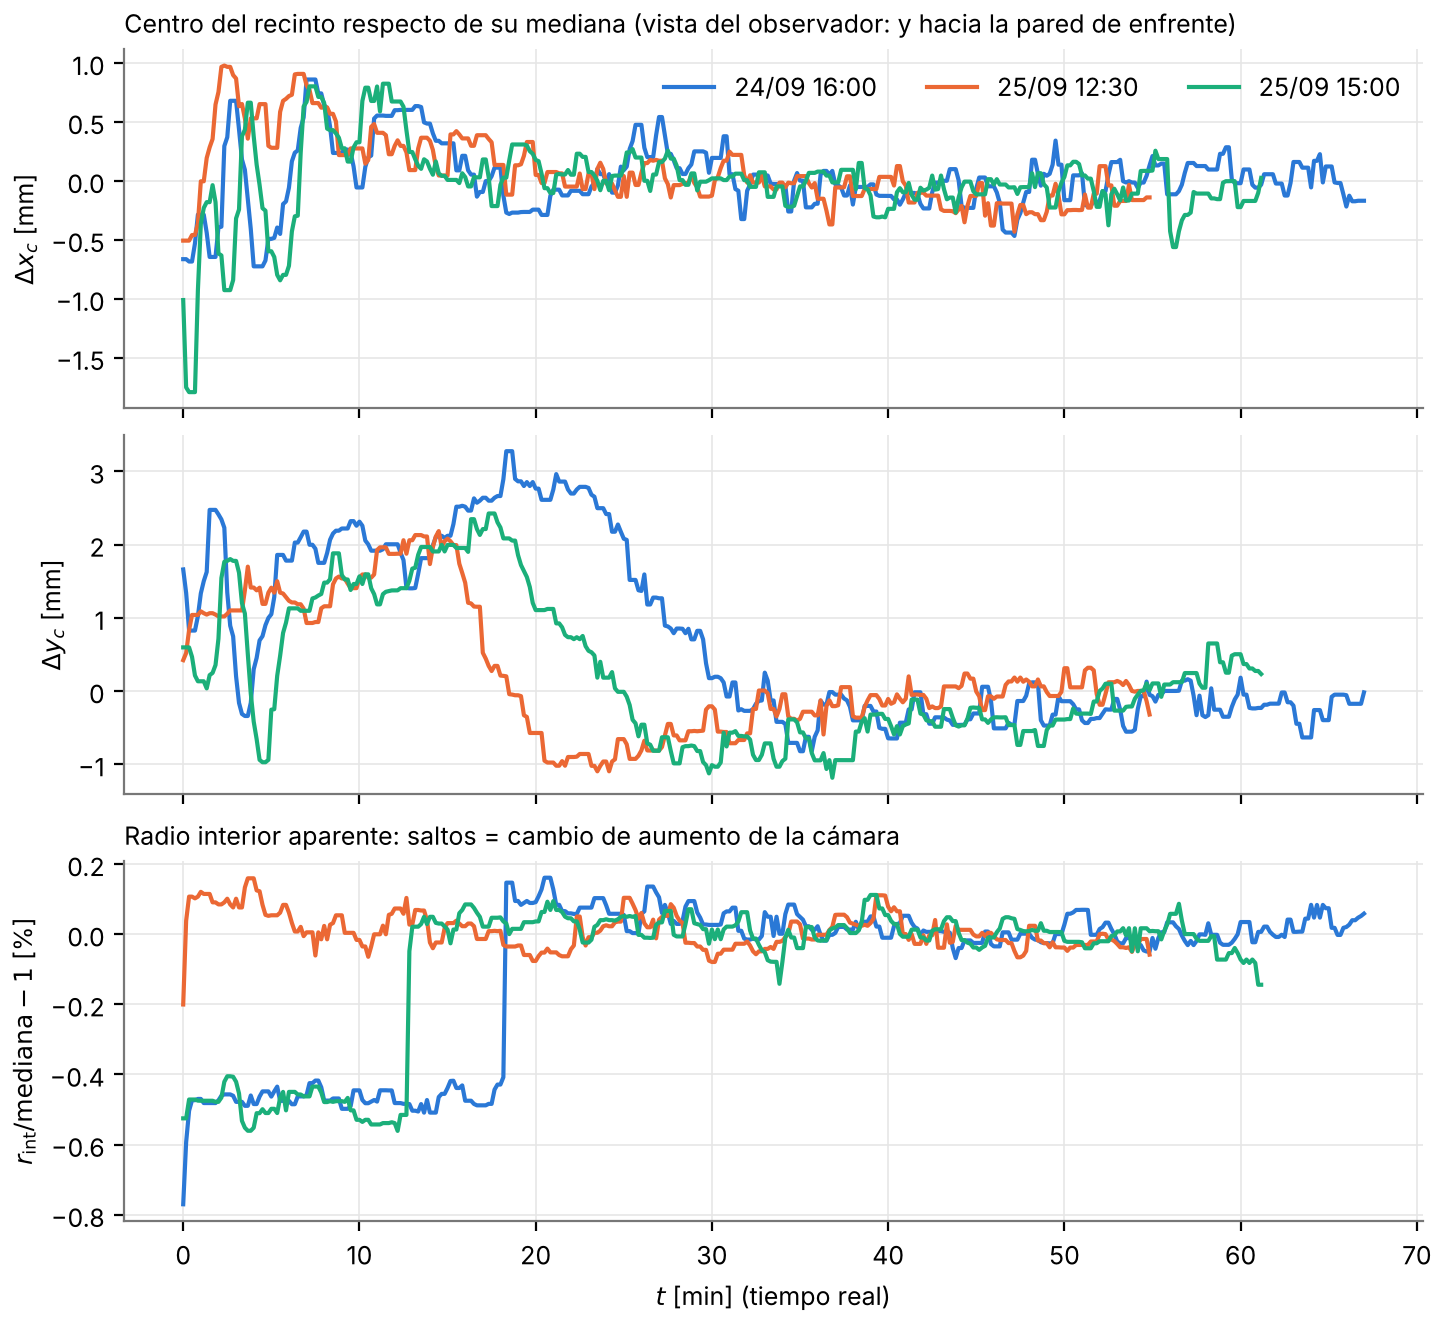
\includegraphics[width=0.95\linewidth]{figuras/recinto_movimiento.png}
  \caption{Centro del recinto (respecto de su mediana, en el sistema de la vista del observador) y radio aparente a lo largo de cada
    ensayo, después de la mediana móvil de 5 muestras. Los saltos del radio coinciden con un agrandamiento
    igual de la placa de fondo: son cambios de aumento de la cámara.}
  \label{fig:recinto_mov}
\end{figure}

\paragraph{La escala es consistente por tres caminos independientes.}
\begin{enumerate}
  \item El cociente de los radios exterior e interior del anillo, que no depende de la escala, coincide
        con $D_{\mathrm{ext}}/D_{\mathrm{int}} = 195/185$ con \SI{0.05}{\percent} (\cref{tab:recinto}).
  \item El cuerpo de los robots (borde de la placa, con LEDs y componentes) mide \SI{101}{px} de
        diámetro en la imagen (mediana sobre \num{4870} rayos sin vecinos en 21 cuadros de \Cmp{Lab}{A};
        rango intercuartil \num{99}--\SI{107}{px}): con $s = \SI{0.323}{\milli\metre\per px}$ son
        \SI{32.7}{\milli\metre}, el diámetro real.
  \item La capa de la pared y la capa media están a \SI{75.2}{} y \SI{42.8}{\milli\metre} del centro en los
        tres ensayos: separadas \SI{32.5}{\milli\metre}, prácticamente un diámetro de robot, como
        corresponde a discos densos apoyados unos en otros.
\end{enumerate}
La escala usada hasta el 07/10 ($s = D/(2\,r_{\mathrm{ext}}) = \SI{0.372}{\milli\metre\per px}$, con
$D = \SI{35}{\milli\metre}$ y el radio del anillo oscuro que usa el detector, $r_{\mathrm{ext}} = \SI{47}{px}$)
no cumple ninguna de las tres: haría que el recinto midiera \SI{213}{\milli\metre} de diámetro y que las
capas estuvieran separadas \SI{37.4}{\milli\metre}, más que un robot. El anillo oscuro es más chico que
el cuerpo del robot. Por eso \textbf{todas las longitudes y velocidades de este informe son
\SI{13}{\percent} menores que en la versión anterior} (factor $0{,}3233/0{,}372 = \num{0.869}$); los
ángulos, $\omega$, los tiempos y los estados de seguimiento no cambian.

\paragraph{Perspectiva.} Los robots apoyados en la pared tienen su centro a $R_{\mathrm{c}} \approx
\SI{78}{\milli\metre}$ del centro, mientras que con $D = \SI{33}{\milli\metre}$ deberían estar a
$R_{\mathrm{int}} - D/2 = \SI{76}{\milli\metre}$. La diferencia (\SI{2.5}{\percent}) es de perspectiva: la
cámara mide el centro del robot en su parte superior y el radio del recinto en el canto del anillo, a
alturas distintas. Se deja sin corregir ($\kappa$ no se aplica) y se toma como incertidumbre sistemática
de las posiciones y velocidades; la aplicación permite aplicarla (\emph{Escala desde: recinto + corrección
de perspectiva}).

\subsection{Escala de tiempo y sincronización con el sensor}\label{sec:escala_ens}

Los videos son \emph{time-lapse}: cada cuadro se toma cada $1/\fr$ segundos reales y el archivo se
reproduce a \SI{29.97}{cuadros\per\second}, unas 10 veces más rápido. Todos los tiempos, velocidades
y velocidades angulares de este informe están en tiempo real con $\fr = 3$~cuadros/s. El valor se
verificó de tres maneras independientes:
\begin{enumerate}
  \item \textbf{Configuración de la cámara}: un \emph{time-lapse} $\times 10$ a \SI{29.97}{cuadros\per\second}
        da $\fr = \num{2.997}$.
  \item \textbf{Duración del registro del sensor}, grabado en simultáneo con su propio reloj
        (\cref{tab:videos}).
  \item \textbf{Correlación con el sensor}: al barrer $\fr$ entre \num{2.985} y \num{3.015}, la correlación
        entre la movilidad de los robots y la señal del sensor es máxima entre \num{2.9975} y \num{3.0025}
        en los tres ensayos (\cref{sec:presion}).
\end{enumerate}
La duración nominal del nombre (\SI{60}{\minute}) \emph{no} sirve para calcular $\fr$: daría valores
entre \num{2.75} y \num{3.36}, con errores de hasta \SI{12}{\percent} en todas las velocidades.

\begin{table}[H]
  \centering
  \caption{Cuadros de los originales (\texttt{VR}) y frecuencia de captura deducida de tres maneras.
    Duración del sensor: $t_{\text{último}} - t_{\text{primero}}$ de \texttt{R\_<código>.csv}; como el
    registro empieza antes que el video, el $\fr$ que da es una cota inferior.}
  \label{tab:videos}
  \small
  \begin{tabular}{@{}lrrrrrr@{}}
    \toprule
    & & \multicolumn{2}{c}{$T$ con $\fr = \num{2.997}$} & \multicolumn{2}{c}{Sensor de presión} & Nominal \\
    \cmidrule(lr){3-4}\cmidrule(lr){5-6}\cmidrule(l){7-7}
    Ensayo & Cuadros & video [\si{\second}] & real [\si{\minute}] & $T$ [\si{\second}] & $\fr$ & $\fr$ (\SI{60}{\minute}) \\
    \midrule
    \Cmp{Lab}{A} & \num{12105} & \num{403.9} & \num{67.3} & \num{4055.1} & \num{2.985} & \num{3.36} \\
    \Cmp{Lab}{B} & \num{9907}  & \num{330.6} & \num{55.1} & \num{3368.4} & \num{2.941} & \num{2.75} \\
    \Cmp{Lab}{C} & \num{11038} & \num{368.3} & \num{61.4} & \num{3699.5} & \num{2.984} & \num{3.07} \\
    \bottomrule
  \end{tabular}
\end{table}

\paragraph{Sincronización.} El registrador del sensor enciende un LED durante \SI{5}{\second} al
comenzar (columna \texttt{LED}). En los tres ensayos, el primer cuadro del video recortado
(\texttt{VC}) coincide con el \emph{fin} de ese pulso: la correlación cruzada entre video y sensor,
calculada sin usar el LED, da el mismo desfasaje con diferencias de \SI{\Cmp{LagLed}{A}}{\second},
\SI{\Cmp{LagLed}{B}}{\second} y \SI{\Cmp{LagLed}{C}}{\second}, menores que dos cuadros. Por lo tanto,
el tiempo del sensor se pasa al del video con
\begin{equation}
  t_{\mathrm{video}} = t_{\mathrm{sensor}} - t_{\mathrm{LED,fin}},
\end{equation}
con $t_{\mathrm{LED,fin}}$ = \SI{\Cmp{LedFin}{A}}{\second}, \SI{\Cmp{LedFin}{B}}{\second} y
\SI{\Cmp{LedFin}{C}}{\second} desde el inicio de cada registro.

% ============================================================================
% Tests report: tracking quality.
% ============================================================================
\section{Calidad del seguimiento}\label{sec:calidad}

Los tres ensayos se siguieron completos, con los 22 robots en todos los cuadros: no quedó ninguna
posición predicha ni perdida, y el \SI{99.9}{\percent} de los puntos se detectó con el umbral
estricto (\cref{tab:calidad}). Los errores se corrigieron a mano con anclas; las advertencias se
revisaron visualmente y, por ser pocas y breves, se dejaron como están. Parte de ellas se debe a un
obstáculo que cruza la escena durante un intervalo corto del ensayo, que no afecta al resto de la
medición.

\begin{table}[H]
  \centering
  \caption{Estados de las posiciones. Un \emph{episodio} es un grupo de cuadros seguidos (separados por
    menos de \Cuadros{3}) con al menos un robot no detectado con el umbral estricto.}
  \label{tab:calidad}
  \small
  \begin{tabular}{@{}lrrr@{}}
    \toprule
    & \Cmp{Lab}{A} & \Cmp{Lab}{B} & \Cmp{Lab}{C} \\
    \midrule
    Puntos (robots $\times$ cuadros) & \num{265518} & \num{217382} & \num{242264} \\
    Detectados con umbral estricto & \num{265298} & \num{217149} & \num{241966} \\
    Detectados con umbral relajado & \num{\Cmp{Rel}{A}} & \num{\Cmp{Rel}{B}} & \num{\Cmp{Rel}{C}} \\
    Interpolados & \num{\Cmp{Int}{A}} & \num{\Cmp{Int}{B}} & \num{\Cmp{Int}{C}} \\
    Anclas manuales & \num{\Cmp{Man}{A}} & \num{\Cmp{Man}{B}} & \num{\Cmp{Man}{C}} \\
    Predichos o perdidos & \num{\Cmp{Pre}{A}} & \num{\Cmp{Pre}{B}} & \num{\Cmp{Pre}{C}} \\
    \midrule
    Episodios con advertencias & 46 & 32 & 16 \\
    Cuadros afectados & \SI{1.81}{\percent} & \SI{2.22}{\percent} & \SI{2.69}{\percent} \\
    Episodio más largo & \SI{16}{\second} & \SI{11}{\second} & \SI{52}{\second} \\
    Robots involucrados & 11 & 7 & 5 \\
    Rotación medida (no interpolada) & \SI{100}{\percent} & \SI{99.99}{\percent} & \SI{100}{\percent} \\
    \bottomrule
  \end{tabular}
\end{table}

Las tres anclas manuales están en los últimos cuadros de \Cmp{Lab}{B} (robot 17, cuadros 9874 y
9875) y de \Cmp{Lab}{C} (robot 19, cuadro 11007). El episodio más largo, en \Cmp{Lab}{C} entre
\SI{19.2}{\minute} y \SI{20.1}{\minute}, es un único robot (el 20) detectado con umbral relajado,
con coberturas del anillo de \num{0.73} a \num{0.78}: su anillo se veía parcialmente tapado, pero la
posición es correcta. Como todos los puntos quedan con su estado en la columna \texttt{status},
pueden excluirse en cualquier análisis sensible; con menos del \SI{0.13}{\percent} de puntos
afectados, incluirlos no cambia ningún resultado de este informe.


\IfFileExists{generado/comparacion/comparacion.tex}{%
  \section{Comparación de los tres ensayos}\label{sec:comparacion}
  Todas las magnitudes están en tiempo real ($\fr = \num{\CuadrosPorSegundo}$~cuadros/s) y en SI
  (escala de cada ensayo en la \cref{tab:config}); los ángulos son positivos en sentido antihorario
  en la arena vista desde arriba ($x$ a la derecha del observador, $y$ hacia la pared de enfrente). Se usan todos
  los puntos con posición observada.
  % Generated by comparar_ensayos.py -- do not edit; re-run the script instead.
\subsection{Tabla comparativa}
\begin{table}[H]
  \centering
  \caption{Comparación de los ensayos: datos, calidad del seguimiento, movimiento y rotación.}
  \label{tab:comparacion}
  \small
  \begin{tabular}{@{}lrrr@{}}
    \toprule
    & \Cmp{Lab}{A} & \Cmp{Lab}{B} & \Cmp{Lab}{C} \\
    \midrule
    \multicolumn{4}{@{}l}{\textit{Ensayo}} \\
    Robots $N$ & \num{\Cmp{N}{A}} & \num{\Cmp{N}{B}} & \num{\Cmp{N}{C}} \\
    Cuadros & \num{\Cmp{F}{A}} & \num{\Cmp{F}{B}} & \num{\Cmp{F}{C}} \\
    Duración real [\si{\minute}] & \num{\Cmp{Dur}{A}} & \num{\Cmp{Dur}{B}} & \num{\Cmp{Dur}{C}} \\
    Escala $s$ [\si{\milli\metre\per px}] & \num{\Cmp{Esc}{A}} & \num{\Cmp{Esc}{B}} & \num{\Cmp{Esc}{C}} \\
    Radio útil de la arena [\si{\centi\metre}] & \num{\Cmp{Rar}{A}} & \num{\Cmp{Rar}{B}} & \num{\Cmp{Rar}{C}} \\
    Fracción de área $\phi$ & \num{\Cmp{Phi}{A}} & \num{\Cmp{Phi}{B}} & \num{\Cmp{Phi}{C}} \\
    \midrule
    \multicolumn{4}{@{}l}{\textit{Seguimiento}} \\
    Posiciones observadas [\si{\percent}] & \num{\Cmp{Obs}{A}} & \num{\Cmp{Obs}{B}} & \num{\Cmp{Obs}{C}} \\
    Puntos con umbral relajado & \num{\Cmp{Rel}{A}} & \num{\Cmp{Rel}{B}} & \num{\Cmp{Rel}{C}} \\
    Puntos interpolados & \num{\Cmp{Int}{A}} & \num{\Cmp{Int}{B}} & \num{\Cmp{Int}{C}} \\
    Anclas manuales & \num{\Cmp{Man}{A}} & \num{\Cmp{Man}{B}} & \num{\Cmp{Man}{C}} \\
    Puntos predichos o perdidos & \num{\Cmp{Pre}{A}} & \num{\Cmp{Pre}{B}} & \num{\Cmp{Pre}{C}} \\
    \midrule
    \multicolumn{4}{@{}l}{\textit{Traslación}} \\
    $|\vec v|$ mediana [\si{\milli\metre\per\second}] & \num{\Cmp{Vmed}{A}} & \num{\Cmp{Vmed}{B}} & \num{\Cmp{Vmed}{C}} \\
    $|\vec v|$ media [\si{\milli\metre\per\second}] & \num{\Cmp{Vmean}{A}} & \num{\Cmp{Vmean}{B}} & \num{\Cmp{Vmean}{C}} \\
    $|\vec v|$ percentil 95 [\si{\milli\metre\per\second}] & \num{\Cmp{Vp95}{A}} & \num{\Cmp{Vp95}{B}} & \num{\Cmp{Vp95}{C}} \\
    $|\vec v|$ mediana fuera de atascos [\si{\milli\metre\per\second}] & \num{\Cmp{VmedAct}{A}} & \num{\Cmp{VmedAct}{B}} & \num{\Cmp{VmedAct}{C}} \\
    Exponente MSD $\alpha$ (1--20 s) & \num{\Cmp{Alfa}{A}} & \num{\Cmp{Alfa}{B}} & \num{\Cmp{Alfa}{C}} \\
    \midrule
    \multicolumn{4}{@{}l}{\textit{Rotación}} \\
    $|\omega|$ mediana [\si{\degree\per\second}] & \num{\Cmp{Wmed}{A}} & \num{\Cmp{Wmed}{B}} & \num{\Cmp{Wmed}{C}} \\
    $\omega$ media (con signo) [\si{\degree\per\second}] & \num{\Cmp{Wmean}{A}} & \num{\Cmp{Wmean}{B}} & \num{\Cmp{Wmean}{C}} \\
    Puntos con $\omega>0$ (antihorario) [\si{\percent}] & \num{\Cmp{Wpos}{A}} & \num{\Cmp{Wpos}{B}} & \num{\Cmp{Wpos}{C}} \\
    Robots con giro neto $>+1$ vuelta & \num{\Cmp{Nccw}{A}} & \num{\Cmp{Nccw}{B}} & \num{\Cmp{Nccw}{C}} \\
    Robots con giro neto $<-1$ vuelta & \num{\Cmp{Ncw}{A}} & \num{\Cmp{Ncw}{B}} & \num{\Cmp{Ncw}{C}} \\
    Mayor giro neto de un robot [\si{vueltas}] & \num{\Cmp{Vmax}{A}} & \num{\Cmp{Vmax}{B}} & \num{\Cmp{Vmax}{C}} \\
    Rotación colectiva $\overline{\Phi}$ & \num{\Cmp{Prot}{A}} & \num{\Cmp{Prot}{B}} & \num{\Cmp{Prot}{C}} \\
    \midrule
    \multicolumn{4}{@{}l}{\textit{Atascos}} \\
    Episodios & \num{\Cmp{NAt}{A}} & \num{\Cmp{NAt}{B}} & \num{\Cmp{NAt}{C}} \\
    Tiempo total [\si{\minute}] & \num{\Cmp{TAt}{A}} & \num{\Cmp{TAt}{B}} & \num{\Cmp{TAt}{C}} \\
    Fracción del ensayo [\si{\percent}] & \num{\Cmp{PAt}{A}} & \num{\Cmp{PAt}{B}} & \num{\Cmp{PAt}{C}} \\
    Episodio más largo [\si{\second}] & \num{\Cmp{AtMax}{A}} & \num{\Cmp{AtMax}{B}} & \num{\Cmp{AtMax}{C}} \\
    \bottomrule
  \end{tabular}
\end{table}
\subsection{Rapidez en el tiempo y atascos}\label{sec:cmp_atascos}
\begin{figure}[H]
  \centering
  \begin{tikzpicture}
    \begin{axis}[width=0.96\linewidth, height=3.6cm, ymin=0, ymax=8, enlarge x limits=false, xmin=0, ylabel={$|\vec v|$ [\si{\milli\metre\per\second}]}, grid=major, grid style={gray!20}, legend style={font=\footnotesize}, tick label style={font=\footnotesize}, title={\Cmp{Lab}{A}}, title style={font=\small, yshift=-1ex}]
      \addplot [ybar interval, fill=gray!30, draw=none, forget plot] table [x=t, y expr=8*\thisrow{atasco}, col sep=comma] {generado/comparacion/serie_A.csv};
      \addplot [azul, thick] table [x=t, y=v_p90, col sep=comma] {generado/comparacion/serie_A.csv};
      \addplot [black, thin] table [x=t, y=v_med, col sep=comma] {generado/comparacion/serie_A.csv};
    \end{axis}
  \end{tikzpicture}

  \begin{tikzpicture}
    \begin{axis}[width=0.96\linewidth, height=3.6cm, ymin=0, ymax=8, enlarge x limits=false, xmin=0, ylabel={$|\vec v|$ [\si{\milli\metre\per\second}]}, grid=major, grid style={gray!20}, legend style={font=\footnotesize}, tick label style={font=\footnotesize}, title={\Cmp{Lab}{B}}, title style={font=\small, yshift=-1ex}]
      \addplot [ybar interval, fill=gray!30, draw=none, forget plot] table [x=t, y expr=8*\thisrow{atasco}, col sep=comma] {generado/comparacion/serie_B.csv};
      \addplot [rojo, thick] table [x=t, y=v_p90, col sep=comma] {generado/comparacion/serie_B.csv};
      \addplot [black, thin] table [x=t, y=v_med, col sep=comma] {generado/comparacion/serie_B.csv};
    \end{axis}
  \end{tikzpicture}

  \begin{tikzpicture}
    \begin{axis}[width=0.96\linewidth, height=3.6cm, ymin=0, ymax=8, enlarge x limits=false, xmin=0, ylabel={$|\vec v|$ [\si{\milli\metre\per\second}]}, grid=major, grid style={gray!20}, legend style={font=\footnotesize}, tick label style={font=\footnotesize}, title={\Cmp{Lab}{C}}, title style={font=\small, yshift=-1ex}, xlabel={$t$ [\si{\minute}]}]
      \addplot [ybar interval, fill=gray!30, draw=none, forget plot] table [x=t, y expr=8*\thisrow{atasco}, col sep=comma] {generado/comparacion/serie_C.csv};
      \addplot [verde, thick] table [x=t, y=v_p90, col sep=comma] {generado/comparacion/serie_C.csv};
      \addplot [black, thin] table [x=t, y=v_med, col sep=comma] {generado/comparacion/serie_C.csv};
    \end{axis}
  \end{tikzpicture}

  \caption{Evolución de la rapidez en ventanas de \SI{30}{\second}: percentil 90 entre robots (color) y mediana (negro). Sombreado: atascos (percentil 90 suavizado $<\SI{\CmpUmbralAtasco}{\milli\metre\per\second}$ durante al menos \SI{\CmpMinAtasco}{\second}).}
  \label{fig:cmp_serie}
\end{figure}
\subsection{Distribuciones}
\begin{figure}[H]
  \centering
  \begin{tikzpicture}
    \begin{axis}[width=0.49\linewidth, height=5.2cm, ymode=log, xmin=0, xmax=8, ymin=1e-4, xlabel={$|\vec v|$ [\si{\milli\metre\per\second}]}, ylabel={densidad [\si{\second\per\milli\metre}]}, grid=major, grid style={gray!20}, legend style={font=\footnotesize}, tick label style={font=\footnotesize}, legend pos=north east]
      \addplot [azul, thick, const plot mark left] table [x=v, y=p, col sep=comma] {generado/comparacion/hist_v_A.csv};
      \addlegendentry{\Cmp{Lab}{A}}
      \addplot [rojo, thick, const plot mark left] table [x=v, y=p, col sep=comma] {generado/comparacion/hist_v_B.csv};
      \addlegendentry{\Cmp{Lab}{B}}
      \addplot [verde, thick, const plot mark left] table [x=v, y=p, col sep=comma] {generado/comparacion/hist_v_C.csv};
      \addlegendentry{\Cmp{Lab}{C}}
    \end{axis}
  \end{tikzpicture}
  \hfill
  \begin{tikzpicture}
    \begin{axis}[width=0.49\linewidth, height=5.2cm, ymode=log, xmin=-60, xmax=60, ymin=1e-4, xlabel={$\omega$ [\si{\degree\per\second}]}, ylabel={densidad [\si{\second\per\degree}]}, grid=major, grid style={gray!20}, legend style={font=\footnotesize}, tick label style={font=\footnotesize}, legend pos=north east]
      \addplot [azul, thick, const plot mark left] table [x=w, y=p, col sep=comma] {generado/comparacion/hist_w_A.csv};
      \addplot [rojo, thick, const plot mark left] table [x=w, y=p, col sep=comma] {generado/comparacion/hist_w_B.csv};
      \addplot [verde, thick, const plot mark left] table [x=w, y=p, col sep=comma] {generado/comparacion/hist_w_C.csv};
    \end{axis}
  \end{tikzpicture}
  \caption{Distribuciones de la rapidez (izq.) y de la velocidad angular (der., positivo = antihorario) de todos los robots y cuadros con posición observada. Escala logarítmica.}
  \label{fig:cmp_hist}
\end{figure}
\subsection{Rotación individual y desplazamiento}
\begin{figure}[H]
  \centering
  \begin{tikzpicture}
    \begin{axis}[width=0.49\linewidth, height=5.2cm, xlabel={robots ordenados por $\overline{\omega}$}, ylabel={$\overline{\omega}$ por robot [\si{\degree\per\second}]}, grid=major, grid style={gray!20}, legend style={font=\footnotesize}, tick label style={font=\footnotesize}, legend pos=south east, xmin=-0.5, xmax=21.5]
      \addplot [azul, thick, mark=*, mark size=1.2pt] table [x=rank, y=w, col sep=comma] {generado/comparacion/giro_A.csv};
      \addlegendentry{\Cmp{Lab}{A}}
      \addplot [rojo, thick, mark=*, mark size=1.2pt] table [x=rank, y=w, col sep=comma] {generado/comparacion/giro_B.csv};
      \addlegendentry{\Cmp{Lab}{B}}
      \addplot [verde, thick, mark=*, mark size=1.2pt] table [x=rank, y=w, col sep=comma] {generado/comparacion/giro_C.csv};
      \addlegendentry{\Cmp{Lab}{C}}
      \addplot [black, thin, forget plot] coordinates {(-1,0) (40,0)};
    \end{axis}
  \end{tikzpicture}
  \hfill
  \begin{tikzpicture}
    \begin{axis}[width=0.49\linewidth, height=5.2cm, xmode=log, ymode=log, xlabel={$\tau$ [\si{\second}]}, ylabel={MSD [\si{\milli\metre\squared}]}, grid=major, grid style={gray!20}, legend style={font=\footnotesize}, tick label style={font=\footnotesize}, legend pos=south east]
      \addplot [azul, thick] table [x=tau, y=msd, col sep=comma] {generado/comparacion/msd_A.csv};
      \addplot [rojo, thick] table [x=tau, y=msd, col sep=comma] {generado/comparacion/msd_B.csv};
      \addplot [verde, thick] table [x=tau, y=msd, col sep=comma] {generado/comparacion/msd_C.csv};
      \addplot [black, dashed, domain=1:20, forget plot] {3*x^2};
      \node[font=\scriptsize, anchor=west] at (axis cs:22,1200) {$\propto\tau^2$};
    \end{axis}
  \end{tikzpicture}
  \caption{Izq.: velocidad angular media de cada robot, ordenada (cada punto es un robot). Der.: desplazamiento cuadrático medio $\mathrm{MSD}(\tau)=\langle|\vec r(t+\tau)-\vec r(t)|^2\rangle$; la recta de referencia indica movimiento balístico.}
  \label{fig:cmp_giro}
\end{figure}
\subsection{Ocupación de la arena}
\begin{figure}[H]
  \centering
  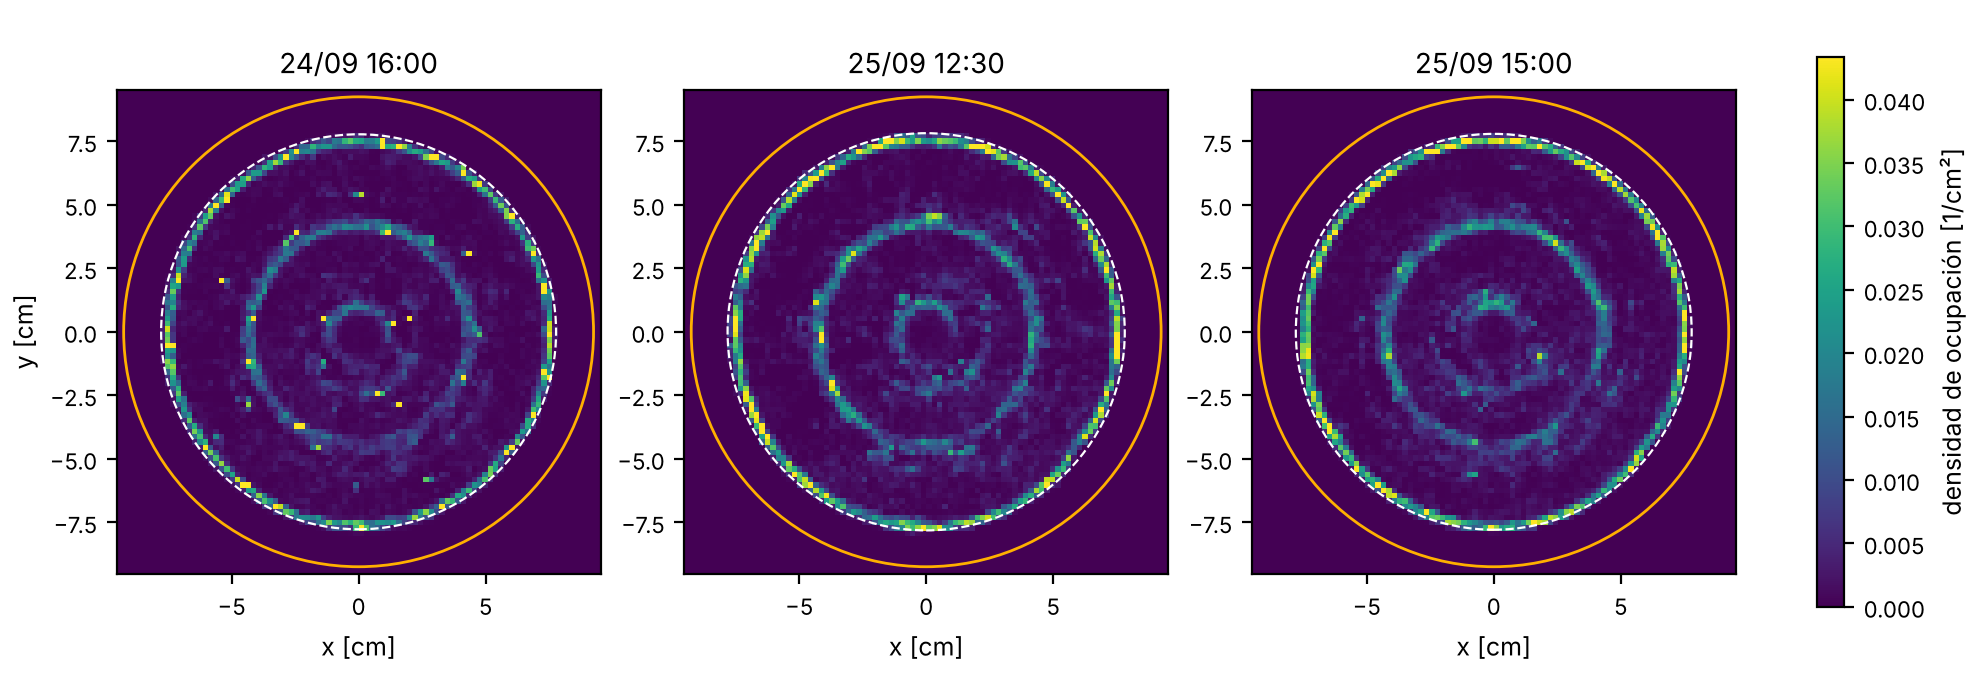
\includegraphics[width=\linewidth]{generado/comparacion/ocupacion.png}
  \caption{Densidad de ocupación de los centros de los robots durante todo cada ensayo. Línea punteada: círculo que pueden alcanzar los centros (radio útil menos el radio del robot).}
  \label{fig:cmp_ocupacion}
\end{figure}
\begin{figure}[H]
  \centering
  \begin{tikzpicture}
    \begin{axis}[width=0.62\linewidth, height=5cm, xmin=0, xmax=1, ymin=0, xlabel={$r/R_{\mathrm{c}}$}, ylabel={densidad relativa}, grid=major, grid style={gray!20}, legend style={font=\footnotesize}, tick label style={font=\footnotesize}, legend pos=north west]
      \addplot [azul, thick, mark=*, mark size=1pt] table [x=r, y=n, col sep=comma] {generado/comparacion/radial_A.csv};
      \addlegendentry{\Cmp{Lab}{A}}
      \addplot [rojo, thick, mark=*, mark size=1pt] table [x=r, y=n, col sep=comma] {generado/comparacion/radial_B.csv};
      \addlegendentry{\Cmp{Lab}{B}}
      \addplot [verde, thick, mark=*, mark size=1pt] table [x=r, y=n, col sep=comma] {generado/comparacion/radial_C.csv};
      \addlegendentry{\Cmp{Lab}{C}}
      \addplot [black, dashed, forget plot] coordinates {(0,1) (1,1)};
    \end{axis}
  \end{tikzpicture}
  \caption{Densidad radial de los centros normalizada por área ($1$ = distribución uniforme); $R_{\mathrm{c}}$ es el radio máximo que alcanzan los centros.}
  \label{fig:cmp_radial}
\end{figure}

  % ============================================================================
% Tests report: interpretation of the comparison (numbers from generado/comparacion/datos.tex).
% ============================================================================
\subsection{Lo observado}\label{sec:observado}

\paragraph{Los tres ensayos son reproducibles.} Con la misma cantidad de robots, la misma arena y el
mismo modo, las tres salidas dan estadísticas muy parecidas (\cref{tab:comparacion}): rapidez mediana
de \num{\Cmp{Vmed}{A}} a \SI{\Cmp{Vmed}{C}}{\milli\metre\per\second}, media de
\num{\Cmp{Vmean}{A}} a \SI{\Cmp{Vmean}{C}}{\milli\metre\per\second} y percentil 95 entre
\num{\Cmp{Vp95}{B}} y \SI{\Cmp{Vp95}{A}}{\milli\metre\per\second}; las distribuciones de rapidez y de
$\omega$ prácticamente se superponen (\cref{fig:cmp_hist}). La diferencia más grande entre ensayos no
está en cómo se mueven los robots cuando se mueven, sino en cuánto tiempo pasan atascados.

\paragraph{El movimiento es intermitente.} El percentil 95 de la rapidez es de cinco a seis veces la
mediana: la mayor parte del tiempo los robots apenas se desplazan (empujados por sus vecinos) y el
desplazamiento ocurre en episodios cortos de \num{3} a \SI{8}{\milli\metre\per\second}. A escalas de
1 a \SI{20}{\second}, el desplazamiento cuadrático medio crece como $\tau^{\alpha}$ con
$\alpha \approx \num{\Cmp{Alfa}{C}}$--$\num{\Cmp{Alfa}{A}}$, entre difusivo ($\alpha=1$) y balístico
($\alpha=2$): los robots mantienen la dirección durante algunos segundos. A tiempos largos el MSD se
satura (\cref{fig:cmp_giro}), porque el confinamiento limita el desplazamiento a la escala de la arena.

\paragraph{Sentido de giro y corrección del espejado.} Los videos están grabados espejados respecto del
eje vertical de la imagen, por lo que un giro horario real se ve antihorario. Todos los datos de este
informe están corregidos (opción \emph{Video espejado: horizontal} de VidFetch): ángulos y posiciones
corresponden a la arena vista desde arriba, con giros positivos en sentido antihorario.

\paragraph{La rotación propia domina.} Todos los robots giran sobre sí mismos de forma persistente:
la $|\omega|$ mediana es de \num{\Cmp{Wmed}{A}} a \SI{\Cmp{Wmed}{B}}{\degree\per\second} y el robot
más rápido acumula \num{\Cmp{Vmax}{C}} vueltas en \SI{\Cmp{Dur}{C}}{\minute} (una $|\overline{\omega}|$
de \SI{\Cmp{Spin}{C}}{\degree\per\second}). En el modo \texttt{QR} todos los robots están programados
para girar a la derecha (sentido horario), y eso es lo que hace la mayoría: en los tres ensayos,
\Cmp{Ncw}{A} robots giraron en neto en sentido horario y el giro medio con signo es negativo, de
\num{\Cmp{Wmean}{B}} a \SI{\Cmp{Wmean}{C}}{\degree\per\second}.

\paragraph{Contrarrotación de los robots de la pared.} Los otros \Cmp{Nccw}{A} robots terminan con un
giro neto antihorario, contrario al programado (\cref{fig:cmp_giro}, izquierda). No son simplemente
robots que fallan: giran despacio ($|\overline{\omega}| \approx \SI{2}{\degree\per\second}$, contra
\num{5}--\SI{6}{\degree\per\second} de los que giran a la derecha), alternan ambos sentidos (giran a la
derecha el \num{40}--\SI{47}{\percent} del tiempo) y pasan más tiempo contra la pared
(\num{58}--\SI{68}{\percent} del tiempo con $r/R_{\mathrm{c}} > 0{,}85$, contra \num{47}--\SI{52}{\percent}).
Esto es lo que se espera de un disco que rueda por el interior de la pared: si avanza en sentido
horario alrededor del centro de la arena apoyado en ella, el rozamiento en el punto de contacto lo hace
girar en sentido antihorario sobre sí mismo, y ese arrastre puede superar al giro propio del motor.
La coincidencia 14/8 en los tres ensayos sugiere además que la tendencia depende de cada robot (por
ejemplo, de la fuerza de su motor); para confirmarlo haría falta identificar a cada robot entre videos,
cosa que el seguimiento no hace.

\paragraph{Hay una circulación colectiva débil.} El parámetro
$\Phi = \langle \hat r_i \times \hat v_i \rangle$ (seno del ángulo entre la posición respecto del
centro de la arena y la velocidad, promediado sobre los robots que se mueven a más de
\SI{1}{\milli\metre\per\second}) vale \num{\Cmp{Prot}{A}}, \num{\Cmp{Prot}{B}} y \num{\Cmp{Prot}{C}}:
valdría $-1$ si todos circularan en sentido horario alrededor del centro, $+1$ en sentido antihorario
y 0 si no hubiera sentido preferido. El grupo circula lentamente en sentido horario, el mismo sentido
del giro programado, con una velocidad angular colectiva de unos \SI{0.2}{\degree\per\second} (una
vuelta cada \SI{30}{\minute}).

\paragraph{Los robots se ordenan en capas.} Los mapas de ocupación (\cref{fig:cmp_ocupacion}) y la
densidad radial (\cref{fig:cmp_radial}) muestran tres anillos concéntricos en $r/R_{\mathrm{c}} \approx
0{,}14$, $0{,}55$ y $0{,}95$, separados por aproximadamente un diámetro de robot. La capa exterior,
apoyada en la pared, es la más poblada; entre la capa media y la exterior la densidad cae a
\num{0.15}--\num{0.4} veces el valor uniforme. Es el ordenamiento esperado de discos densos en un recinto circular ($\phi \approx 0{,}58$):
los robots se reacomodan dentro de cada capa y pasan poco tiempo entre capas.

\paragraph{Atascos.} Los tres ensayos tienen intervalos en los que todo el grupo se detiene
(\cref{fig:cmp_serie,fig:atascos}): la rapidez de casi todos los robots cae al nivel del ruido de posición
(mediana $\approx\SI{0.2}{\milli\metre\per\second}$) y la rotación propia también se frena, de
$|\omega| \approx \SI{4}{\degree\per\second}$ a menos de \SI{1.5}{\degree\per\second}. No es una pausa de los
robots: siguen encendidos (los LEDs se ven en el video) y el movimiento se reanuda solo. \Cmp{Lab}{A} es
el ensayo más afectado: \Cmp{NAt}{A} atascos que suman \SI{\Cmp{TAt}{A}}{\minute}
(\SI{\Cmp{PAt}{A}}{\percent} del ensayo), uno de \SI{\Cmp{AtMax}{A}}{\second} entre los minutos 45 y 51,
y otro que dura desde el minuto 62 hasta el final. \Cmp{Lab}{B} tuvo un único atasco de
\SI{\Cmp{AtMax}{B}}{\second} y \Cmp{Lab}{C}, \Cmp{NAt}{C} cortos (\SI{\Cmp{TAt}{C}}{\minute} en total).
Fuera de los atascos, la rapidez mediana de los tres ensayos es casi igual
(\num{\Cmp{VmedAct}{B}}--\SI{\Cmp{VmedAct}{C}}{\milli\metre\per\second}).

\begin{figure}[H]
  \centering
  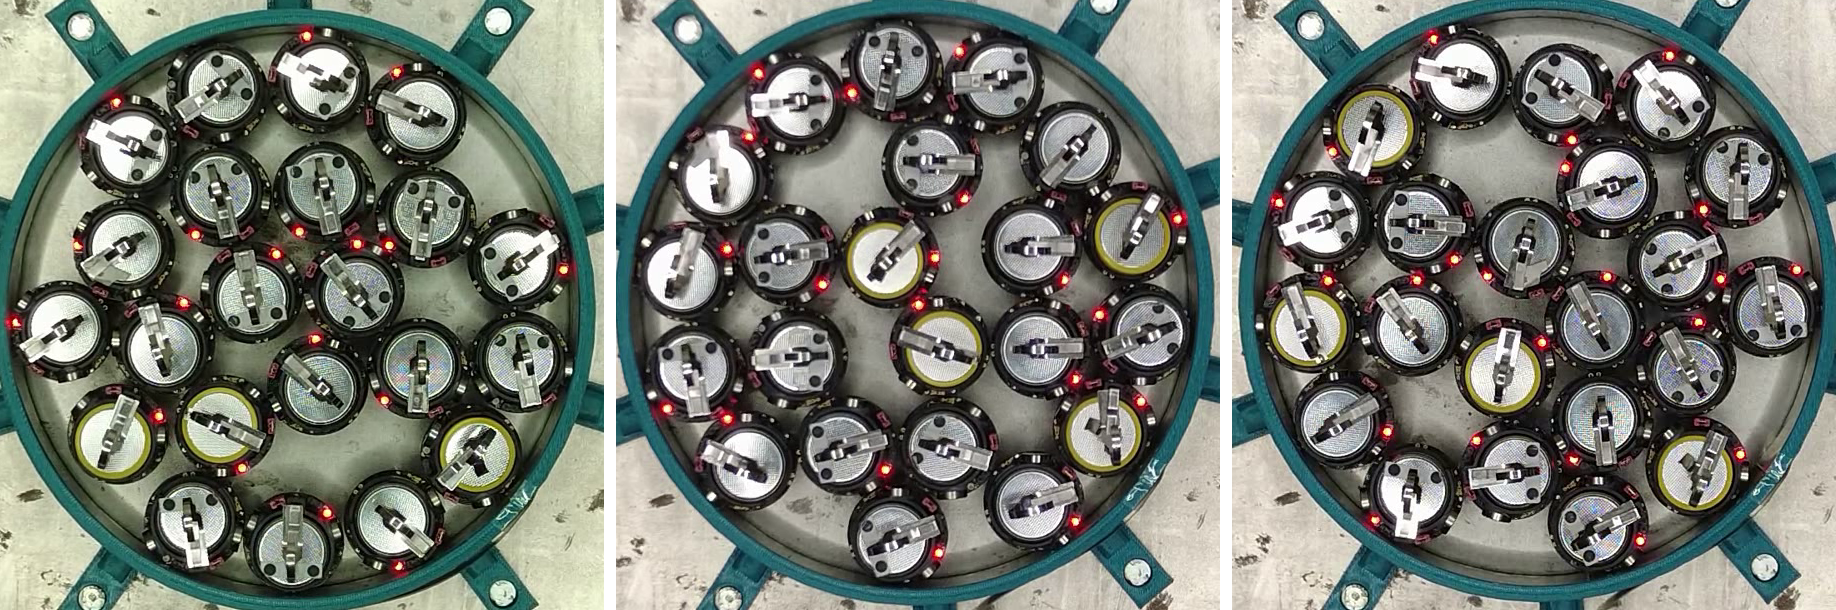
\includegraphics[width=\linewidth]{figuras/atascos.png}
  \caption{Un cuadro durante el atasco principal de cada ensayo (de izquierda a derecha: \Cmp{Lab}{A},
    minuto 47,8; \Cmp{Lab}{B}, minuto 50,6; \Cmp{Lab}{C}, minuto 19,7). Imágenes tal como las graba la cámara (espejadas). Los robots siguen
    encendidos (LEDs rojos), pero durante el atasco prácticamente no se desplazan ni giran.}
  \label{fig:atascos}
\end{figure}

  % ============================================================================
% Tests report: exploratory link between video and pressure sensor.
% ============================================================================
\section{Contraste con el sensor de presión}\label{sec:presion}

Cada ensayo se registró también con el sensor de fuerza (FSR) del proyecto. Se usa su conductancia
$G = 1/R_{\mathrm{FSR}}$, que crece con la fuerza aplicada, y se la alinea con el video mediante el
pulso LED de sincronización (\cref{sec:escala_ens}). Este contraste es exploratorio: se compara la
\emph{movilidad} medida en el video (percentil 90 de la rapidez de los 22 robots) con la señal del
sensor, sin un modelo de cómo se transmite la fuerza hasta él.

\IfFileExists{generado/comparacion/presion.tex}{% Generated by comparar_ensayos.py
\begin{table}[H]
  \centering
  \caption{Alineación del registro de presión con el video y conductancia dentro y fuera de los atascos.}
  \label{tab:presion}
  \small
  \begin{tabular}{@{}lrrr@{}}
    \toprule
    & \Cmp{Lab}{A} & \Cmp{Lab}{B} & \Cmp{Lab}{C} \\
    \midrule
    Pulso LED: inicio [\si{\second}] & \num{\Cmp{Led}{A}} & \num{\Cmp{Led}{B}} & \num{\Cmp{Led}{C}} \\
    Pulso LED: fin ($=$ inicio del video) [\si{\second}] & \num{\Cmp{LedFin}{A}} & \num{\Cmp{LedFin}{B}} & \num{\Cmp{LedFin}{C}} \\
    Retardo por correlación cruzada [\si{\second}] & \num{\Cmp{Lag}{A}} & \num{\Cmp{Lag}{B}} & \num{\Cmp{Lag}{C}} \\
    Coeficiente de correlación $r$ & \num{\Cmp{Rxc}{A}} & \num{\Cmp{Rxc}{B}} & \num{\Cmp{Rxc}{C}} \\
    Correlación cruzada $-$ fin del pulso [\si{\second}] & \num{\Cmp{LagLed}{A}} & \num{\Cmp{LagLed}{B}} & \num{\Cmp{LagLed}{C}} \\
    $G$ mediana en atascos [\si{\micro\siemens}] & \num{\Cmp{Gin}{A}} & \num{\Cmp{Gin}{B}} & \num{\Cmp{Gin}{C}} \\
    $G$ mediana fuera de atascos [\si{\micro\siemens}] & \num{\Cmp{Gout}{A}} & \num{\Cmp{Gout}{B}} & \num{\Cmp{Gout}{C}} \\
    Cociente & \num{\Cmp{Grat}{A}} & \num{\Cmp{Grat}{B}} & \num{\Cmp{Grat}{C}} \\
    Muestras saturadas en atascos [\si{\percent}] & \num{\Cmp{SatIn}{A}} & \num{\Cmp{SatIn}{B}} & \num{\Cmp{SatIn}{C}} \\
    Muestras saturadas en total [\si{\percent}] & \num{\Cmp{SatAll}{A}} & \num{\Cmp{SatAll}{B}} & \num{\Cmp{SatAll}{C}} \\
    \bottomrule
  \end{tabular}
\end{table}
\begin{figure}[H]
  \centering
  \begin{tikzpicture}
    \begin{axis}[width=0.93\linewidth, height=3.6cm, axis y line*=left, ymin=0, ymax=8, xmin=0, enlarge x limits=false, ylabel={$|\vec v|_{90}$ [\si{\milli\metre\per\second}]}, grid=major, grid style={gray!20}, legend style={font=\footnotesize}, tick label style={font=\footnotesize}, title={\Cmp{Lab}{A}}, title style={font=\small, yshift=-1ex}]
      \addplot [ybar interval, fill=gray!30, draw=none] table [x=t, y expr=8*\thisrow{atasco}, col sep=comma] {generado/comparacion/presion_A.csv};
      \addplot [azul, thin] table [x=t, y=v_p90, col sep=comma] {generado/comparacion/presion_A.csv};
    \end{axis}
    \begin{axis}[width=0.93\linewidth, height=3.6cm, axis y line*=right, axis x line=none, xmin=0, enlarge x limits=false, ylabel={$\log_{10} G$ [\si{\micro\siemens}]}, ylabel style={rojo}, tick label style={font=\footnotesize}]
      \addplot [rojo, thin] table [x=t, y=logG, col sep=comma] {generado/comparacion/presion_A.csv};
    \end{axis}
  \end{tikzpicture}

  \begin{tikzpicture}
    \begin{axis}[width=0.93\linewidth, height=3.6cm, axis y line*=left, ymin=0, ymax=8, xmin=0, enlarge x limits=false, ylabel={$|\vec v|_{90}$ [\si{\milli\metre\per\second}]}, grid=major, grid style={gray!20}, legend style={font=\footnotesize}, tick label style={font=\footnotesize}, title={\Cmp{Lab}{B}}, title style={font=\small, yshift=-1ex}]
      \addplot [ybar interval, fill=gray!30, draw=none] table [x=t, y expr=8*\thisrow{atasco}, col sep=comma] {generado/comparacion/presion_B.csv};
      \addplot [azul, thin] table [x=t, y=v_p90, col sep=comma] {generado/comparacion/presion_B.csv};
    \end{axis}
    \begin{axis}[width=0.93\linewidth, height=3.6cm, axis y line*=right, axis x line=none, xmin=0, enlarge x limits=false, ylabel={$\log_{10} G$ [\si{\micro\siemens}]}, ylabel style={rojo}, tick label style={font=\footnotesize}]
      \addplot [rojo, thin] table [x=t, y=logG, col sep=comma] {generado/comparacion/presion_B.csv};
    \end{axis}
  \end{tikzpicture}

  \begin{tikzpicture}
    \begin{axis}[width=0.93\linewidth, height=3.6cm, axis y line*=left, ymin=0, ymax=8, xmin=0, enlarge x limits=false, ylabel={$|\vec v|_{90}$ [\si{\milli\metre\per\second}]}, grid=major, grid style={gray!20}, legend style={font=\footnotesize}, tick label style={font=\footnotesize}, title={\Cmp{Lab}{C}}, title style={font=\small, yshift=-1ex}, xlabel={$t$ de video [\si{\minute}]}]
      \addplot [ybar interval, fill=gray!30, draw=none] table [x=t, y expr=8*\thisrow{atasco}, col sep=comma] {generado/comparacion/presion_C.csv};
      \addplot [azul, thin] table [x=t, y=v_p90, col sep=comma] {generado/comparacion/presion_C.csv};
    \end{axis}
    \begin{axis}[width=0.93\linewidth, height=3.6cm, axis y line*=right, axis x line=none, xmin=0, enlarge x limits=false, ylabel={$\log_{10} G$ [\si{\micro\siemens}]}, ylabel style={rojo}, tick label style={font=\footnotesize}]
      \addplot [rojo, thin] table [x=t, y=logG, col sep=comma] {generado/comparacion/presion_C.csv};
    \end{axis}
  \end{tikzpicture}

  \caption{Movilidad de los robots (percentil 90 de la rapidez, azul; atascos sombreados) y conductancia del sensor de presión $G=1/R$ (rojo, escala logarítmica, medianas de \SI{10}{\second}), con el registro alineado al fin del pulso LED de sincronización (\cref{tab:presion}).}
  \label{fig:cmp_presion}
\end{figure}
}{}

\paragraph{Resultado.} En \Cmp{Lab}{A} la relación es directa: los dos atascos largos coinciden con
los intervalos de máxima conductancia (\cref{fig:cmp_presion}). Durante los atascos la mediana de $G$
es de \SI{\Cmp{Gin}{A}}{\micro\siemens}, contra \SI{\Cmp{Gout}{A}}{\micro\siemens} fuera de ellos, y el
\SI{\Cmp{SatIn}{A}}{\percent} de las muestras está saturado (el ADC llega a su máximo, $R_{\mathrm{FSR}}
= \SI{1141.5}{\ohm}$ con la resistencia de realimentación de \SI{5}{\kilo\ohm} que se usaba ese día). El
episodio de saturación de \SI{382}{\second} documentado en el análisis del sensor coincide con el
atasco de \SI{\Cmp{AtMax}{A}}{\second} entre los minutos 45 y 51 del video: la saturación empieza
unos \SI{13}{\second} después de que el grupo se detiene y termina junto con el atasco (dentro de él,
el \SI{96}{\percent} de las muestras está saturado). En los otros dos atascos de \Cmp{Lab}{A} el sensor
no satura, pero su conductancia mediana (\num{87} y \SI{250}{\micro\siemens}) sigue siendo miles de
veces mayor que fuera de los atascos. En \Cmp{Lab}{C} el atasco
principal (minutos 19 a 21) también coincide con un pico de conductancia, con $G$ \Cmp{Grat}{C} veces
mayor en los atascos que fuera de ellos. En \Cmp{Lab}{B}, en cambio, el único atasco no se ve en el
sensor (cociente \num{\Cmp{Grat}{B}}).

\paragraph{Interpretación.} Un atasco es un estado bloqueado: los robots siguen empujando, pero la red
de contactos no les deja lugar para moverse ni girar. Si el sensor queda dentro de esa red de
contactos, recibe una fuerza sostenida y alta; si el bloqueo se forma lejos del sensor, este no lo
registra, como en \Cmp{Lab}{B}. Los picos de $G$ fuera de los atascos (\cref{fig:cmp_presion})
corresponden a contactos transitorios que no llegan a detener a todo el grupo. Para afirmar más que
esta coincidencia haría falta conocer la posición del sensor en la arena y medir qué robots lo
tocan en cada momento, cosa que el video permite si se marca la ubicación del sensor.

}{%
  \section{Comparación de los ensayos}
  Falta ejecutar \texttt{comparar\_ensayos.py} (ver el informe de la aplicación).
}

% ============================================================================
% Tests report: conclusions.
% ============================================================================
\section{Conclusiones}\label{sec:conclusiones}

\begin{itemize}
  \item Los tres ensayos (22 robots, modo \texttt{QR}, $\phi \approx 0{,}58$) se siguieron completos:
        \SI{100}{\percent} de posiciones observadas, menos del \SI{0.13}{\percent} con umbral relajado y
        tres anclas manuales en total.
  \item La escala de tiempo $\fr = 3$~cuadros/s queda verificada por la configuración de la cámara, la
        duración del registro y la correlación con el sensor (máxima entre \num{2.9975} y \num{3.0025}).
        El inicio de cada video recortado coincide con el fin del pulso LED, que sirve de sincronización.
  \item El comportamiento es reproducible: rapidez mediana \num{0.58}--\SI{0.70}{\milli\metre\per\second},
        percentil 95 \num{3.5}--\SI{3.6}{\milli\metre\per\second}, $|\omega|$ mediana
        \num{3.0}--\SI{3.8}{\degree\per\second} y desplazamiento cuadrático medio superdifusivo
        ($\alpha \approx 1{,}3$) en los tres.
  \item Corregido el espejado del video, 14 de 22 robots giran en neto a la derecha (horario), como
        indica el modo \texttt{QR}, y el grupo circula débilmente en ese mismo sentido. Los otros 8
        contrarrotan despacio y pasan más tiempo contra la pared, como un disco que rueda por el interior
        del recinto.
  \item El grupo se ordena en tres capas concéntricas separadas por aproximadamente un diámetro.
  \item Los atascos colectivos son la principal diferencia entre ensayos (\SI{17}{\percent},
        \SI{3}{\percent} y \SI{6}{\percent} del tiempo). En dos de los tres ensayos coinciden con la
        máxima fuerza registrada por el sensor de presión: en \Cmp{Lab}{A}, el atasco de
        \SI{382}{\second} coincide con el episodio de saturación del sensor.
\end{itemize}

\paragraph{Próximos pasos.}
\begin{itemize}
  \item Marcar en el video la posición del sensor y relacionar la fuerza con los robots en contacto
        con él.
  \item Repetir con los otros modos (\texttt{R}, \texttt{QZ}) y con distinta cantidad de robots, para ver
        cómo cambian los atascos con $\phi$.
  \item Identificar a cada robot entre videos (por ejemplo, con marcas de color) para saber si los que
        contrarrotan son siempre los mismos o los que quedan contra la pared.
\end{itemize}


\appendix
\IfFileExists{generado/lista_ensayos.tex}{%
  % Generated by generar_informe.py: one line per processed video.
% Generated by generar_informe.py for VP_20262409_1600_22QR_60_robots.csv. Manual remarks go in notas.tex.
\begingroup
% Generated by generar_informe.py -- do not edit; re-run the script instead.
\def\VTitulo{20262409\_1600\_22QR\_60}
\def\VArchivo{VP\_20262409\_1600\_22QR\_60\_robots.csv}
\def\VVideo{VC\_20262409\_1600\_22QR\_60.MP4}
\def\VFrameIni{0}
\def\VFrameFin{12068}
\def\VCuadros{12069}
\def\VFps{3}
\def\VDuracion{4.02e+03}
\def\VN{22}
\def\VUnidadL{cm}
\def\VUnidadV{mm/s}
\def\VEscala{0.3723}
\def\VEscalaFuente{escala exportada por la app (diámetro real cargado en la pestaña Seguimiento)}
\def\VEscalaQ{\SI{0.3723}{\milli\metre\per px}}
\def\VFpsQ{\num{3} cuadros = \SI{1}{\second} real ($\Delta t = \SI{0.333}{\second}$)}
\def\VDuracionQ{\SI{67}{\minute}}
\def\VRescala{tomada del CSV exportado}
\def\VDiamQ{\SI{35}{\milli\metre} $\equiv$ \SI{94}{px}}
\def\VUL{\centi\metre}
\def\VUV{\milli\metre\per\second}
\def\VDiamMM{35}
\def\VDiamPx{94}
\def\VPctObs{100}
\def\VPctRot{100}
\def\VNErr{0}
\def\VNAdv{0}
\def\VVmedia{1.04}
\def\VVmediana{0.579}
\def\VVpNoventaycinco{3.59}
\def\VRecMedio{513}
\def\VNetoMedio{7.3}

\section{Ensayo \VTitulo}\label{sec:20262409_1600_22QR_60}

\begin{table}[H]
  \centering
  \caption{Datos del ensayo \VTitulo.}
  \begin{tabular}{@{}lp{0.58\linewidth}@{}}
    \toprule
    Archivo de datos & \texttt{\VArchivo} \\
    Video & \texttt{\VVideo} \\
    Cuadros analizados & \VFrameIni\,--\,\VFrameFin{} (\num{\VCuadros}) \\
    Escala de tiempo & \VFpsQ\newline{\footnotesize\VRescala} \\
    Duración real & \VDuracionQ \\
    Robots seguidos ($N$) & \num{\VN} \\
    Diámetro del robot & \VDiamQ \\
    Escala & \VEscalaQ\newline{\footnotesize\VEscalaFuente} \\
    Posiciones observadas & \SI{\VPctObs}{\percent} \\
    Cuadros con error / con advertencia & \num{\VNErr} / \num{\VNAdv} \\
    \bottomrule
  \end{tabular}
\end{table}

\IfFileExists{generado/20262409_1600_22QR_60/captura.png}{%
\begin{figure}[H]
  \centering
  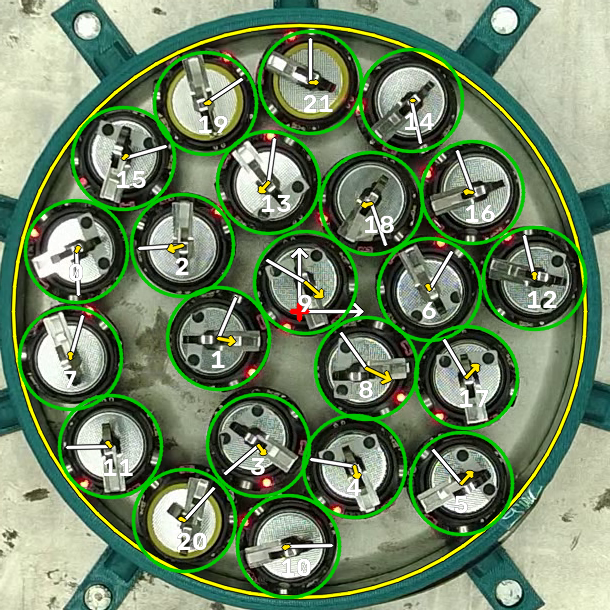
\includegraphics[width=0.62\linewidth]{generado/20262409_1600_22QR_60/captura.png}
  \caption{Cuadro de ejemplo con identificador, vector velocidad (amarillo, largo = desplazamiento en 7,5 cuadros) y orientación (aguja blanca). Círculo verde: posición observada; naranja: estimada. Imagen tal como la graba la cámara (espejada); flecha y aguja dibujadas sobre ella.}
\end{figure}}{}

\begin{figure}[H]
  \centering
  \begin{tikzpicture}
    \begin{axis}[width=0.97\linewidth, height=5.2cm, xlabel={$t$ [\si{\minute}]},
        ylabel={$|\vec v|$ [\si{\milli\metre\per\second}]}, ymin=0, grid=major, grid style={gray!20}, scaled ticks=false, tick label style={/pgf/number format/fixed, /pgf/number format/precision=3},
        legend pos=north east, legend style={font=\footnotesize}, enlarge x limits=false]
      \addplot [name path=q75, draw=none, forget plot] table [x=t, y=v_q75, col sep=comma] {generado/20262409_1600_22QR_60/serie.csv};
      \addplot [name path=q25, draw=none, forget plot] table [x=t, y=v_q25, col sep=comma] {generado/20262409_1600_22QR_60/serie.csv};
      \addplot [azul!25] fill between [of=q25 and q75];
      \addlegendentry{rango intercuartil}
      \addplot [azul, thick] table [x=t, y=v_mean, col sep=comma] {generado/20262409_1600_22QR_60/serie.csv};
      \addlegendentry{media de los $N$ robots}
    \end{axis}
  \end{tikzpicture}
  \caption{Rapidez de los robots en función del tiempo.}
\end{figure}

\begin{figure}[H]
  \centering
  \begin{tikzpicture}
    \begin{axis}[width=0.8\linewidth, height=5cm, xlabel={$|\vec v|$ [\si{\milli\metre\per\second}]},
        ylabel={densidad [\si{\second\per\milli\metre}]},
        ymin=0, enlarge x limits=false, grid=major, grid style={gray!20},
        scaled ticks=false, tick label style={/pgf/number format/fixed, /pgf/number format/precision=3}]
      \addplot [fill=azul!35, draw=azul, const plot mark left] table [x=v, y=dens, col sep=comma] {generado/20262409_1600_22QR_60/hist_v.csv} \closedcycle;
    \end{axis}
  \end{tikzpicture}
  \caption{Distribución de la rapidez (solo posiciones observadas).}
\end{figure}

\begin{figure}[H]
  \centering
  \begin{tikzpicture}
    \begin{axis}[width=0.72\linewidth, axis equal image, y dir=reverse, xlabel={$x$ [\si{\centi\metre}]},
        ylabel={$y$ [\si{\centi\metre}]}, grid=major, grid style={gray!20}, cycle list name=robots,
        tick label style={font=\footnotesize}]
      \pgfplotsinvokeforeach{0,...,21}{%
        \addplot+ [thin, no markers] table [x=x#1, y=y#1, col sep=comma] {generado/20262409_1600_22QR_60/tray.csv};}
    \end{axis}
  \end{tikzpicture}
  \caption{Trayectorias de los 22 robots (escena real, video espejado corregido; $y$ hacia abajo), primeros 5 minutos reales.}
\end{figure}

\begin{figure}[H]
  \centering
  \begin{tikzpicture}
    \begin{axis}[width=0.97\linewidth, height=5.4cm, xlabel={$t$ [\si{\minute}]},
        ylabel={$\theta$ [vueltas]}, grid=major, grid style={gray!20}, cycle list name=robots, enlarge x limits=false]
      \pgfplotsinvokeforeach{0,...,21}{%
        \addplot+ [thin, no markers] table [x=t, y=th#1, col sep=comma] {generado/20262409_1600_22QR_60/theta.csv};}
    \end{axis}
  \end{tikzpicture}
  \caption{Orientación acumulada de cada robot ($\theta=0$ en el primer cuadro; positivo = antihorario).}
\end{figure}

\begin{table}[H]
  \centering
  \caption{Resumen por robot.}
  \footnotesize
  \pgfplotstabletypeset[col sep=comma, columns={id,obs,vmed,vmax,rec,net,vueltas,wabs},
      every head row/.style={before row=\toprule, after row=\midrule}, every last row/.style={after row=\bottomrule},
      columns/id/.style={column name={Robot}, int detect},
      columns/obs/.style={column name={Obs. [\si{\percent}]}, fixed, precision=1},
      columns/vmed/.style={fixed, fixed zerofill, precision=1, column name={$\overline{|\vec v|}$ [\si{\milli\metre\per\second}]}},
      columns/vmax/.style={fixed, fixed zerofill, precision=1, column name={$|\vec v|_{\max}$ [\si{\milli\metre\per\second}]}},
      columns/rec/.style={fixed, fixed zerofill, precision=2, column name={Recorrido [\si{\centi\metre}]}},
      columns/net/.style={fixed, fixed zerofill, precision=2, column name={Despl. neto [\si{\centi\metre}]}}, columns/vueltas/.style={column name={$\theta_{\mathrm{final}}$ [vueltas]}, fixed, precision=2},
      columns/wabs/.style={column name={$\overline{|\omega|}$ [\si{\degree\per\second}]}, fixed, fixed zerofill, precision=1},
    ]{generado/20262409_1600_22QR_60/resumen.csv}
\end{table}

\subsection{Lo observado}
Se siguieron \num{22} robots durante \num{12069} cuadros (\SI{67}{\minute}). El \SI{100}{\percent} de las posiciones fue observado (detectado o corregido a mano); el resto se estimó por interpolación o predicción.
No hubo cuadros con posiciones estimadas.
La rapidez mediana fue \SI{0.579}{\milli\metre\per\second} y el percentil 95, \SI{3.59}{\milli\metre\per\second}: la cola rápida es \num{6.2} veces la mediana, lo que indica movimiento intermitente, con episodios cortos de alta velocidad.
El robot más rápido en promedio fue el \num{6} (\SI{1.46}{\milli\metre\per\second}).
En rotación, \num{8} robots giraron en neto en sentido antihorario, \num{14} en sentido horario y \num{0} giraron menos de media vuelta. El que más giró fue el \num{6}, con $|\omega|$ media de \SI{14.7}{\degree\per\second}. La rotación se midió directamente en el \SI{100}{\percent} de los puntos.

\IfFileExists{generado/20262409_1600_22QR_60/notas.tex}{% Observaciones propias sobre este ensayo (este archivo no se sobrescribe).
% Ejemplo:
% \paragraph{Notas.} A partir de $t\approx\SI{3}{\second}$ los robots se
% agrupan contra la pared norte de la arena.
}{}
\endgroup

% Generated by generar_informe.py for VP_20262509_1230_22QR_60_robots.csv. Manual remarks go in notas.tex.
\begingroup
% Generated by generar_informe.py -- do not edit; re-run the script instead.
\def\VTitulo{20262509\_1230\_22QR\_60}
\def\VArchivo{VP\_20262509\_1230\_22QR\_60\_robots.csv}
\def\VVideo{VC\_20262509\_1230\_22QR\_60.MP4}
\def\VFrameIni{0}
\def\VFrameFin{9880}
\def\VCuadros{9881}
\def\VFps{3}
\def\VDuracion{3.29e+03}
\def\VN{22}
\def\VUnidadL{cm}
\def\VUnidadV{mm/s}
\def\VEscala{0.3723}
\def\VEscalaFuente{escala exportada por la app (diámetro real cargado en la pestaña Seguimiento)}
\def\VEscalaQ{\SI{0.3723}{\milli\metre\per px}}
\def\VFpsQ{\num{3} cuadros = \SI{1}{\second} real ($\Delta t = \SI{0.333}{\second}$)}
\def\VDuracionQ{\SI{54.9}{\minute}}
\def\VRescala{tomada del CSV exportado}
\def\VDiamQ{\SI{35}{\milli\metre} $\equiv$ \SI{94}{px}}
\def\VUL{\centi\metre}
\def\VUV{\milli\metre\per\second}
\def\VDiamMM{35}
\def\VDiamPx{94}
\def\VPctObs{99.99}
\def\VPctRot{99.99}
\def\VNErr{0}
\def\VNAdv{15}
\def\VVmedia{1.05}
\def\VVmediana{0.644}
\def\VVpNoventaycinco{3.5}
\def\VRecMedio{434}
\def\VNetoMedio{10.9}

\section{Ensayo \VTitulo}\label{sec:20262509_1230_22QR_60}

\begin{table}[H]
  \centering
  \caption{Datos del ensayo \VTitulo.}
  \begin{tabular}{@{}lp{0.58\linewidth}@{}}
    \toprule
    Archivo de datos & \texttt{\VArchivo} \\
    Video & \texttt{\VVideo} \\
    Cuadros analizados & \VFrameIni\,--\,\VFrameFin{} (\num{\VCuadros}) \\
    Escala de tiempo & \VFpsQ\newline{\footnotesize\VRescala} \\
    Duración real & \VDuracionQ \\
    Robots seguidos ($N$) & \num{\VN} \\
    Diámetro del robot & \VDiamQ \\
    Escala & \VEscalaQ\newline{\footnotesize\VEscalaFuente} \\
    Origen de coordenadas & \VOrigen \\
    Recinto & \VRecinto \\
    Posiciones observadas & \SI{\VPctObs}{\percent} \\
    Cuadros con error / con advertencia & \num{\VNErr} / \num{\VNAdv} \\
    \bottomrule
  \end{tabular}
\end{table}

\IfFileExists{generado/20262509_1230_22QR_60/captura.png}{%
\begin{figure}[H]
  \centering
  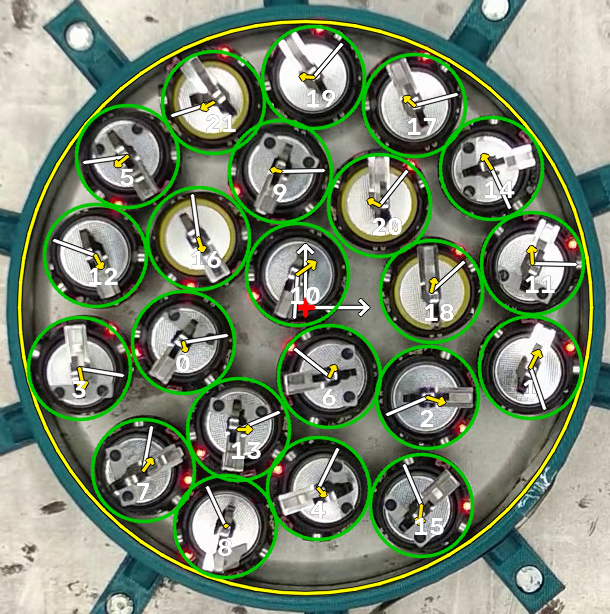
\includegraphics[width=0.62\linewidth]{generado/20262509_1230_22QR_60/captura.png}
  \caption{Cuadro de ejemplo con identificador, vector velocidad (amarillo, largo = desplazamiento en 7,5 cuadros) y orientación (aguja blanca). Círculo verde: posición observada; naranja: estimada. Imagen tal como la graba la cámara (espejada); flecha y aguja dibujadas sobre ella.}
\end{figure}}{}

\begin{figure}[H]
  \centering
  \begin{tikzpicture}
    \begin{axis}[width=0.97\linewidth, height=5.2cm, xlabel={$t$ [\si{\minute}]},
        ylabel={$|\vec v|$ [\si{\milli\metre\per\second}]}, ymin=0, grid=major, grid style={gray!20}, scaled ticks=false, tick label style={/pgf/number format/fixed, /pgf/number format/precision=3},
        legend pos=north east, legend style={font=\footnotesize}, enlarge x limits=false]
      \addplot [name path=q75, draw=none, forget plot] table [x=t, y=v_q75, col sep=comma] {generado/20262509_1230_22QR_60/serie.csv};
      \addplot [name path=q25, draw=none, forget plot] table [x=t, y=v_q25, col sep=comma] {generado/20262509_1230_22QR_60/serie.csv};
      \addplot [azul!25] fill between [of=q25 and q75];
      \addlegendentry{rango intercuartil}
      \addplot [azul, thick] table [x=t, y=v_mean, col sep=comma] {generado/20262509_1230_22QR_60/serie.csv};
      \addlegendentry{media de los $N$ robots}
    \end{axis}
  \end{tikzpicture}
  \caption{Rapidez de los robots en función del tiempo.}
\end{figure}

\begin{figure}[H]
  \centering
  \begin{tikzpicture}
    \begin{axis}[width=0.8\linewidth, height=5cm, xlabel={$|\vec v|$ [\si{\milli\metre\per\second}]},
        ylabel={densidad [\si{\second\per\milli\metre}]},
        ymin=0, enlarge x limits=false, grid=major, grid style={gray!20},
        scaled ticks=false, tick label style={/pgf/number format/fixed, /pgf/number format/precision=3}]
      \addplot [fill=azul!35, draw=azul, const plot mark left] table [x=v, y=dens, col sep=comma] {generado/20262509_1230_22QR_60/hist_v.csv} \closedcycle;
    \end{axis}
  \end{tikzpicture}
  \caption{Distribución de la rapidez (solo posiciones observadas).}
\end{figure}

\begin{figure}[H]
  \centering
  \begin{tikzpicture}
    \begin{axis}[width=0.72\linewidth, axis equal image, xlabel={$x$ [\si{\centi\metre}]},
        ylabel={$y$ [\si{\centi\metre}]}, grid=major, grid style={gray!20}, cycle list name=robots,
        tick label style={font=\footnotesize}]
      \pgfplotsinvokeforeach{0,...,21}{%
        \addplot+ [thin, no markers] table [x=x#1, y=y#1, col sep=comma] {generado/20262509_1230_22QR_60/tray.csv};}
      \draw [gray, thick] (axis cs:0,0) circle [radius=9.25];
      \addplot [only marks, mark=+, mark size=3pt, black] coordinates {(0,0)};
    \end{axis}
  \end{tikzpicture}
  \caption{Trayectorias de los 22 robots (escena real, video espejado corregido; origen en el centro del recinto, $y$ hacia arriba; círculo gris: pared interior), primeros 5 minutos reales.}
\end{figure}

\begin{figure}[H]
  \centering
  \begin{tikzpicture}
    \begin{axis}[width=0.97\linewidth, height=5.4cm, xlabel={$t$ [\si{\minute}]},
        ylabel={$\theta$ [vueltas]}, grid=major, grid style={gray!20}, cycle list name=robots, enlarge x limits=false]
      \pgfplotsinvokeforeach{0,...,21}{%
        \addplot+ [thin, no markers] table [x=t, y=th#1, col sep=comma] {generado/20262509_1230_22QR_60/theta.csv};}
    \end{axis}
  \end{tikzpicture}
  \caption{Orientación acumulada de cada robot ($\theta=0$ en el primer cuadro; positivo = antihorario).}
\end{figure}

\begin{table}[H]
  \centering
  \caption{Resumen por robot.}
  \footnotesize
  \pgfplotstabletypeset[col sep=comma, columns={id,obs,vmed,vmax,rec,net,vueltas,wabs},
      every head row/.style={before row=\toprule, after row=\midrule}, every last row/.style={after row=\bottomrule},
      columns/id/.style={column name={Robot}, int detect},
      columns/obs/.style={column name={Obs. [\si{\percent}]}, fixed, precision=1},
      columns/vmed/.style={fixed, fixed zerofill, precision=2, column name={$\overline{|\vec v|}$ [\si{\milli\metre\per\second}]}},
      columns/vmax/.style={fixed, fixed zerofill, precision=2, column name={$|\vec v|_{\max}$ [\si{\milli\metre\per\second}]}},
      columns/rec/.style={fixed, fixed zerofill, precision=2, column name={Recorrido [\si{\centi\metre}]}},
      columns/net/.style={fixed, fixed zerofill, precision=2, column name={Despl. neto [\si{\centi\metre}]}}, columns/vueltas/.style={column name={$\theta_{\mathrm{final}}$ [vueltas]}, fixed, precision=2},
      columns/wabs/.style={column name={$\overline{|\omega|}$ [\si{\degree\per\second}]}, fixed, fixed zerofill, precision=1},
    ]{generado/20262509_1230_22QR_60/resumen.csv}
\end{table}

\subsection{Lo observado}
Se siguieron \num{22} robots durante \num{9881} cuadros (\SI{54.9}{\minute}). El \SI{99.99}{\percent} de las posiciones fue observado (detectado o corregido a mano); el resto se estimó por interpolación o predicción.
Hubo \num{0} cuadros con posiciones predichas o perdidas y \num{15} cuadros con posiciones interpoladas; conviene excluirlos de los análisis sensibles usando la columna \texttt{status}.
La rapidez mediana fue \SI{0.561}{\milli\metre\per\second} y el percentil 95, \SI{3.05}{\milli\metre\per\second}: la cola rápida es \num{5.4} veces la mediana, lo que indica movimiento intermitente, con episodios cortos de alta velocidad.
El robot más rápido en promedio fue el \num{6} (\SI{1.58}{\milli\metre\per\second}).
En rotación, \num{8} robots giraron en neto en sentido antihorario, \num{14} en sentido horario y \num{0} giraron menos de media vuelta. El que más giró fue el \num{6}, con $|\omega|$ media de \SI{15.4}{\degree\per\second}. La rotación se midió directamente en el \SI{99.99}{\percent} de los puntos.

\IfFileExists{generado/20262509_1230_22QR_60/notas.tex}{% Observaciones propias sobre este ensayo (este archivo no se sobrescribe).
% Ejemplo:
% \paragraph{Notas.} A partir de $t\approx\SI{3}{\second}$ los robots se
% agrupan contra la pared norte de la arena.
}{}
\endgroup

% Generated by generar_informe.py for VP_20262509_1500_22QR_60_robots.csv. Manual remarks go in notas.tex.
\begingroup
% Generated by generar_informe.py -- do not edit; re-run the script instead.
\def\VTitulo{20262509\_1500\_22QR\_60}
\def\VArchivo{VP\_20262509\_1500\_22QR\_60\_robots.csv}
\def\VVideo{VC\_20262509\_1500\_22QR\_60.MP4}
\def\VFrameIni{0}
\def\VFrameFin{11011}
\def\VCuadros{11012}
\def\VFps{3}
\def\VDuracion{3.67e+03}
\def\VN{22}
\def\VUnidadL{cm}
\def\VUnidadV{mm/s}
\def\VEscala{0.3715}
\def\VEscalaFuente{escala exportada por la app (diámetro real cargado en la pestaña Seguimiento)}
\def\VEscalaQ{\SI{0.3715}{\milli\metre\per px}}
\def\VFpsQ{\num{3} cuadros = \SI{1}{\second} real ($\Delta t = \SI{0.333}{\second}$)}
\def\VDuracionQ{\SI{61.2}{\minute}}
\def\VRescala{tomada del CSV exportado}
\def\VDiamQ{\SI{35}{\milli\metre} $\equiv$ \SI{94.2}{px}}
\def\VUL{\centi\metre}
\def\VUV{\milli\metre\per\second}
\def\VDiamMM{35}
\def\VDiamPx{94.2}
\def\VPctObs{100}
\def\VPctRot{100}
\def\VNErr{0}
\def\VNAdv{0}
\def\VVmedia{1.1}
\def\VVmediana{0.697}
\def\VVpNoventaycinco{3.55}
\def\VRecMedio{486}
\def\VNetoMedio{10.9}

\section{Ensayo \VTitulo}\label{sec:20262509_1500_22QR_60}

\begin{table}[H]
  \centering
  \caption{Datos del ensayo \VTitulo.}
  \begin{tabular}{@{}lp{0.58\linewidth}@{}}
    \toprule
    Archivo de datos & \texttt{\VArchivo} \\
    Video & \texttt{\VVideo} \\
    Cuadros analizados & \VFrameIni\,--\,\VFrameFin{} (\num{\VCuadros}) \\
    Escala de tiempo & \VFpsQ\newline{\footnotesize\VRescala} \\
    Duración real & \VDuracionQ \\
    Robots seguidos ($N$) & \num{\VN} \\
    Diámetro del robot & \VDiamQ \\
    Escala & \VEscalaQ\newline{\footnotesize\VEscalaFuente} \\
    Origen de coordenadas & \VOrigen \\
    Recinto & \VRecinto \\
    Posiciones observadas & \SI{\VPctObs}{\percent} \\
    Cuadros con error / con advertencia & \num{\VNErr} / \num{\VNAdv} \\
    \bottomrule
  \end{tabular}
\end{table}

\IfFileExists{generado/20262509_1500_22QR_60/captura.png}{%
\begin{figure}[H]
  \centering
  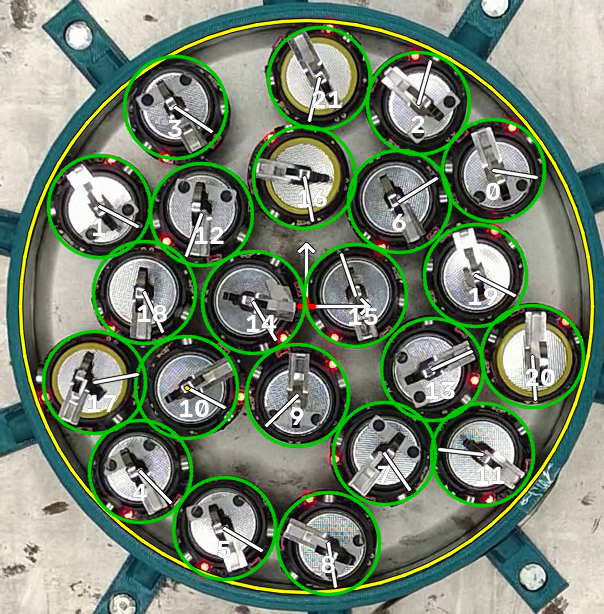
\includegraphics[width=0.62\linewidth]{generado/20262509_1500_22QR_60/captura.png}
  \caption{Cuadro de ejemplo con identificador, vector velocidad (amarillo, largo = desplazamiento en 7,5 cuadros) y orientación (aguja blanca). Círculo verde: posición observada; naranja: estimada. Imagen rotada 180° (vista del observador): $x$ a la derecha, $y$ hacia arriba (lejos del observador).}
\end{figure}}{}

\begin{figure}[H]
  \centering
  \begin{tikzpicture}
    \begin{axis}[width=0.97\linewidth, height=5.2cm, xlabel={$t$ [\si{\minute}]},
        ylabel={$|\vec v|$ [\si{\milli\metre\per\second}]}, ymin=0, grid=major, grid style={gray!20}, scaled ticks=false, tick label style={/pgf/number format/fixed, /pgf/number format/precision=3},
        legend pos=north east, legend style={font=\footnotesize}, enlarge x limits=false]
      \addplot [name path=q75, draw=none, forget plot] table [x=t, y=v_q75, col sep=comma] {generado/20262509_1500_22QR_60/serie.csv};
      \addplot [name path=q25, draw=none, forget plot] table [x=t, y=v_q25, col sep=comma] {generado/20262509_1500_22QR_60/serie.csv};
      \addplot [azul!25] fill between [of=q25 and q75];
      \addlegendentry{rango intercuartil}
      \addplot [azul, thick] table [x=t, y=v_mean, col sep=comma] {generado/20262509_1500_22QR_60/serie.csv};
      \addlegendentry{media de los $N$ robots}
    \end{axis}
  \end{tikzpicture}
  \caption{Rapidez de los robots en función del tiempo.}
\end{figure}

\begin{figure}[H]
  \centering
  \begin{tikzpicture}
    \begin{axis}[width=0.8\linewidth, height=5cm, xlabel={$|\vec v|$ [\si{\milli\metre\per\second}]},
        ylabel={densidad [\si{\second\per\milli\metre}]},
        ymin=0, enlarge x limits=false, grid=major, grid style={gray!20},
        scaled ticks=false, tick label style={/pgf/number format/fixed, /pgf/number format/precision=3}]
      \addplot [fill=azul!35, draw=azul, const plot mark left] table [x=v, y=dens, col sep=comma] {generado/20262509_1500_22QR_60/hist_v.csv} \closedcycle;
    \end{axis}
  \end{tikzpicture}
  \caption{Distribución de la rapidez (solo posiciones observadas).}
\end{figure}

\begin{figure}[H]
  \centering
  \begin{tikzpicture}
    \begin{axis}[width=0.72\linewidth, axis equal image, xlabel={$x$ [\si{\centi\metre}]},
        ylabel={$y$ [\si{\centi\metre}]}, grid=major, grid style={gray!20}, cycle list name=robots,
        tick label style={font=\footnotesize}]
      \pgfplotsinvokeforeach{0,...,21}{%
        \addplot+ [thin, no markers] table [x=x#1, y=y#1, col sep=comma] {generado/20262509_1500_22QR_60/tray.csv};}
      \draw [gray, thick] (axis cs:0,0) circle [radius=9.25];
      \addplot [only marks, mark=+, mark size=3pt, black] coordinates {(0,0)};
    \end{axis}
  \end{tikzpicture}
  \caption{Trayectorias de los 22 robots (imagen rotada 180° (vista del observador); origen en el centro del recinto, $y$ hacia arriba; círculo gris: pared interior), primeros 5 minutos reales.}
\end{figure}

\begin{figure}[H]
  \centering
  \begin{tikzpicture}
    \begin{axis}[width=0.97\linewidth, height=5.4cm, xlabel={$t$ [\si{\minute}]},
        ylabel={$\theta$ [vueltas]}, grid=major, grid style={gray!20}, cycle list name=robots, enlarge x limits=false]
      \pgfplotsinvokeforeach{0,...,21}{%
        \addplot+ [thin, no markers] table [x=t, y=th#1, col sep=comma] {generado/20262509_1500_22QR_60/theta.csv};}
    \end{axis}
  \end{tikzpicture}
  \caption{Orientación acumulada de cada robot ($\theta=0$ en el primer cuadro; positivo = antihorario).}
\end{figure}

\begin{table}[H]
  \centering
  \caption{Resumen por robot.}
  \footnotesize
  \pgfplotstabletypeset[col sep=comma, columns={id,obs,vmed,vmax,rec,net,vueltas,wabs},
      every head row/.style={before row=\toprule, after row=\midrule}, every last row/.style={after row=\bottomrule},
      columns/id/.style={column name={Robot}, int detect},
      columns/obs/.style={column name={Obs. [\si{\percent}]}, fixed, precision=1},
      columns/vmed/.style={fixed, fixed zerofill, precision=2, column name={$\overline{|\vec v|}$ [\si{\milli\metre\per\second}]}},
      columns/vmax/.style={fixed, fixed zerofill, precision=2, column name={$|\vec v|_{\max}$ [\si{\milli\metre\per\second}]}},
      columns/rec/.style={fixed, fixed zerofill, precision=2, column name={Recorrido [\si{\centi\metre}]}},
      columns/net/.style={fixed, fixed zerofill, precision=2, column name={Despl. neto [\si{\centi\metre}]}}, columns/vueltas/.style={column name={$\theta_{\mathrm{final}}$ [vueltas]}, fixed, precision=2},
      columns/wabs/.style={column name={$\overline{|\omega|}$ [\si{\degree\per\second}]}, fixed, fixed zerofill, precision=1},
    ]{generado/20262509_1500_22QR_60/resumen.csv}
\end{table}

\subsection{Lo observado}
Se siguieron \num{22} robots durante \num{11012} cuadros (\SI{61.2}{\minute}). El \SI{100}{\percent} de las posiciones fue observado (detectado o corregido a mano); el resto se estimó por interpolación o predicción.
No hubo cuadros con posiciones estimadas.
La rapidez mediana fue \SI{0.606}{\milli\metre\per\second} y el percentil 95, \SI{3.09}{\milli\metre\per\second}: la cola rápida es \num{5.1} veces la mediana, lo que indica movimiento intermitente, con episodios cortos de alta velocidad.
El robot más rápido en promedio fue el \num{3} (\SI{1.78}{\milli\metre\per\second}).
En rotación, \num{14} robots giraron en neto en sentido antihorario, \num{8} en sentido horario y \num{0} giraron menos de media vuelta. El que más giró fue el \num{3}, con $|\omega|$ media de \SI{23.6}{\degree\per\second}. La rotación se midió directamente en el \SI{100}{\percent} de los puntos.

\IfFileExists{generado/20262509_1500_22QR_60/notas.tex}{% Observaciones propias sobre este ensayo (este archivo no se sobrescribe).
% Ejemplo:
% \paragraph{Notas.} A partir de $t\approx\SI{3}{\second}$ los robots se
% agrupan contra la pared norte de la arena.
}{}
\endgroup

%
}{%
  \section{Resultados por ensayo}
  Todavía no se procesó ningún ensayo con \texttt{generar\_informe.py}.
}

\end{document}
